%%%%%%%%%%%%%%%%%%%%%%%%%%%%%%
%%%%%%%%%%%%%%%%%%%%%%%%%%%%%%

% To use this template, copy and paste the Template folder found here an place within the folder your beamer presentation is located.
% Make sure to include the following code as the first two lines of your document:
% \documentclass[compress]{beamer}
% \ProvidesPackageRCS $Header: SDAL_Beamer.sty ,v 1 05/13/2016 $

\mode<presentation>

% Set presentation size

\usepackage[orientation=landscape,size=custom,width=16,height=9,scale=0.5,debug]{beamerposter} 
\setbeamersize{text margin left=.25in,text margin right=.25in}

% Set Fonts

%\usepackage[T1]{fontenc}
%\usepackage[default]{raleway}
 
 \usefonttheme{serif}
 
 \setbeamerfont{frametitle}{series=\bfseries} 
\setbeamerfont{title}{series=\bfseries} 
\setbeamerfont{author}{series=\bfseries} 

%\usepackage[T1]{fontenc}
%\usepackage[nosfdefault]{raleway}

% Set the size of the font

\usepackage{scrextend}
\changefontsizes{14pt}
\setbeamerfont{title}{size=\fontsize{17pt}{17pt}}
\setbeamerfont{author}{size=\fontsize{14pt}{14pt}}
\setbeamerfont{frametitle}{size=\fontsize{17pt}{17pt}}
\setbeamerfont{date}{size=\fontsize{14pt}{14pt}}
\setbeamerfont*{structure}{size*={17pt}{17pt}}
\setbeamerfont*{tiny structure}{size*={6pt}{6pt}}
  
% Table of Contents

\setbeamertemplate{section in toc}[ball]
\setbeamertemplate{subsection in toc}[square]

\setbeamertemplate{subsection in toc}{\hspace{1.2em}{\color{BIlightblue}\rule[0.3ex]{6pt}{6pt}}~\inserttocsubsection\par}

% Set Color

\definecolor{VTmaroon}{RGB}{102,0,0} 
\definecolor{VTorange}{RGB}{255,102,0}
\definecolor{BIdarkblue}{RGB}{18,37,45}
\definecolor{BIaquablue}{RGB}{126,168,173}
\definecolor{BIcoolgrey}{RGB}{153,153,153}
\definecolor{BIlightblue}{RGB}{93,137,180}
\definecolor{BIlightgreen}{RGB}{141,194,136}

 
\setbeamercolor*{title}{fg=black}
\setbeamercolor{author}{fg=black} 
\setbeamercolor{frametitle}{fg=black} 
\setbeamercolor{section in toc}{fg=black}
\setbeamercolor{subsection in toc}{fg=black}
\setbeamercolor{itemize subsubitem}{fg=black}
\setbeamercolor{itemize subitem}{fg=black}
\setbeamercolor{itemize item}{fg=black}
\setbeamercolor{section number projected}{bg=BIlightblue,fg=white}

% Lists

\makeatletter
\renewcommand{\itemize}[1][]{%
  \beamer@ifempty{#1}{}{\def\beamer@defaultospec{#1}}%
  \ifnum \@itemdepth >2\relax\@toodeep\else
    \advance\@itemdepth\@ne
    \beamer@computepref\@itemdepth% sets \beameritemnestingprefix
    \usebeamerfont{itemize/enumerate \beameritemnestingprefix body}%
    \usebeamercolor[fg]{itemize/enumerate \beameritemnestingprefix body}%
    \usebeamertemplate{itemize/enumerate \beameritemnestingprefix body begin}%
    \list
      {\usebeamertemplate{itemize \beameritemnestingprefix item}}
      {%
        \setlength\topsep{0pt}%NEW
        \setlength\partopsep{0pt}%NEW
        \setlength\itemsep{0pt}%NEW
        \def\makelabel##1{%
          {%
            \hss\llap{{%
                \usebeamerfont*{itemize \beameritemnestingprefix item}%
                \usebeamercolor[fg]{itemize \beameritemnestingprefix item}##1}}%
          }%
        }%
      }
  \fi%
  \beamer@cramped%
  \raggedright%
  \beamer@firstlineitemizeunskip%
}
\makeatother

\setlength\topsep{-10pt}
\setlength\partopsep{-10pt}


\setbeamertemplate{itemize items}[circle]
\setbeamertemplate{itemize subitem}{---}
\setbeamertemplate{itemize subsubitem}[circle]

% TOC

\makeatletter
\patchcmd{\beamer@sectionintoc}
  {\vfill}
  {\vskip\itemsep}
  {}
  {}
\makeatother  

% Remove navigation symbols

\setbeamertemplate{navigation symbols}{}

% Format Title Page

\defbeamertemplate*{title page}{customized}[1][]
{
\centering
\vspace{.9in}\hspace*{-3.8in}
\begin{overlayarea}{4.1in}{1cm}
\centering{
\usebeamerfont{title}\inserttitle\par}
\usebeamerfont{subtitle}\usebeamercolor[fg]{subtitle}\insertsubtitle\par
\end{overlayarea}\\
\vspace{.2in}\hspace*{-1in}
\begin{overlayarea}{4in}{1cm}
\centering{
\usebeamerfont{date}\insertdate\par \vspace{.1in}
\usebeamerfont{author}\insertauthor\par
\usebeamerfont{institute}\insertinstitute\par}
\end{overlayarea}
}

%%% Formatting Different Frame Styles

% Title

\makeatletter
\define@key{beamerframe}{Title}[true]{%
\usebackgroundtemplate{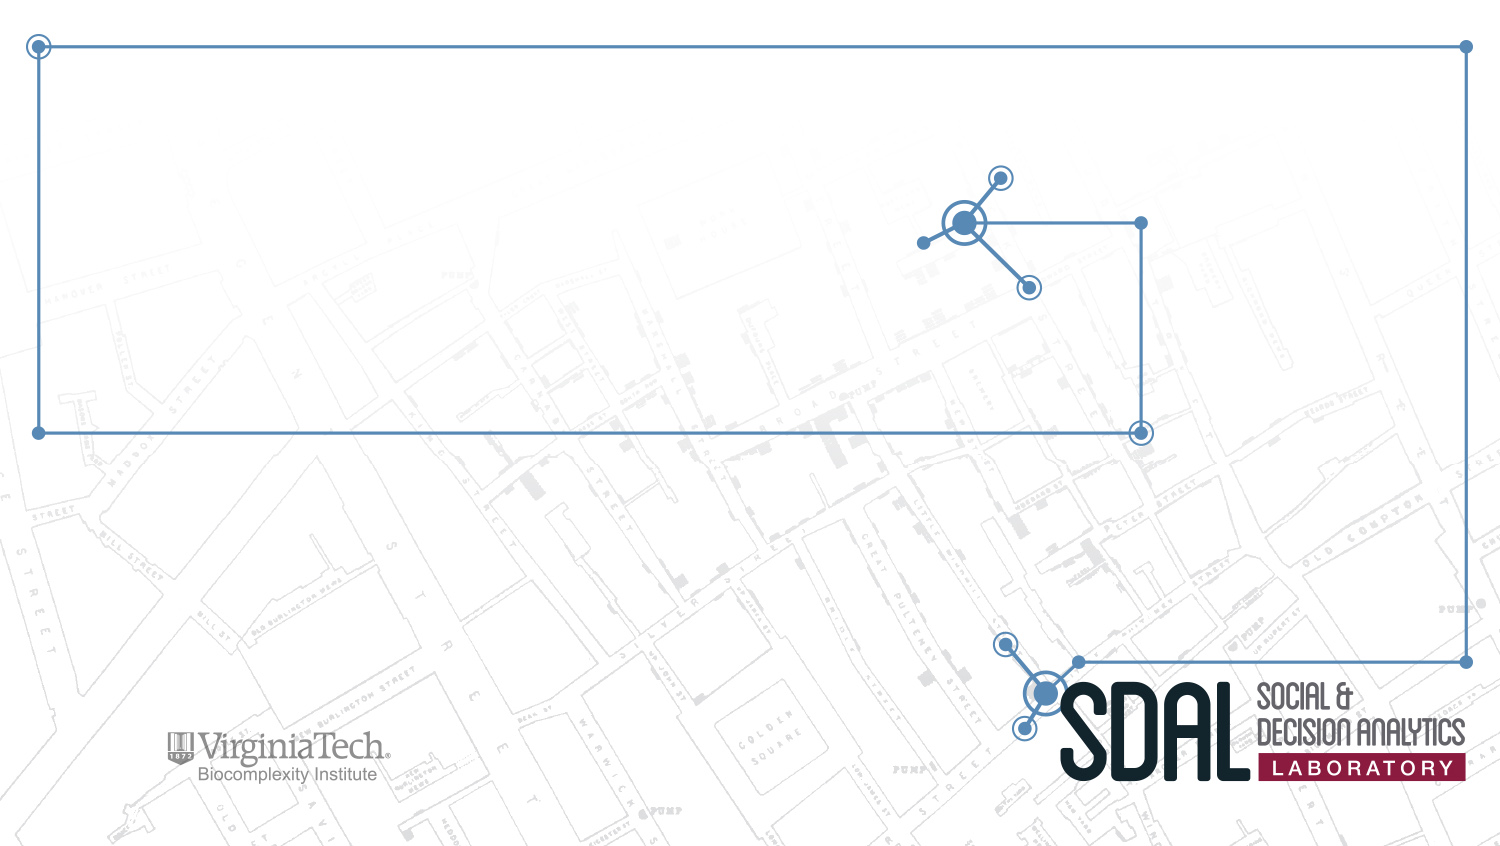
\includegraphics[height=\paperheight,width=\paperwidth]{Template/slides/Title.jpg}
\setbeamertemplate{frametitle}[default][right]
\addtobeamertemplate{frametitle}{\vskip.1in\hspace*{.5in}}{}}
\setbeamertemplate{footline}{}
}
\makeatother

% Outline

\makeatletter
\define@key{beamerframe}{ToC}[true]{%
\usebackgroundtemplate{
\includegraphics[height=\paperheight,width=\paperwidth]{Template/slides/Blank.jpg}}
\setbeamertemplate{frametitle}[default][right]
\addtobeamertemplate{frametitle}{\vskip.1in\hspace*{.5in}}{}
\setbeamertemplate{footline}{}
}
\makeatother

% Blank

\makeatletter
\define@key{beamerframe}{Blank}[true]{%
\usebackgroundtemplate{
\includegraphics[height=\paperheight,width=\paperwidth]{Template/slides/Blank.jpg}}
\setbeamertemplate{frametitle}
{\begin{flushright}\vspace{.23in}{\insertframetitle\hspace{.2in}}\end{flushright}}
\setbeamertemplate{footline}{%
\leavevmode%
  \hbox{%
    \begin{beamercolorbox}[wd=\paperwidth,ht=2.5ex,dp=1.125ex]{palette quaternary}%
    \vspace{.08in}\insertnavigation{\paperwidth}{}{\hskip0pt plus1filll}
    \end{beamercolorbox}%
  }
}
}
\makeatother

% BlankLogo

\makeatletter
\define@key{beamerframe}{BlankLogo}[true]{%
\usebackgroundtemplate{
\includegraphics[height=\paperheight,width=\paperwidth]{Template/slides/BlankLogo.jpg}}
\setbeamertemplate{frametitle}
{\begin{flushright}\vspace{.23in}{\insertframetitle\hspace{.2in}}\end{flushright}}
\setbeamertemplate{footline}{}
}
\makeatother

% Basic1

\makeatletter
\define@key{beamerframe}{Basic1}[true]{%
\usebackgroundtemplate{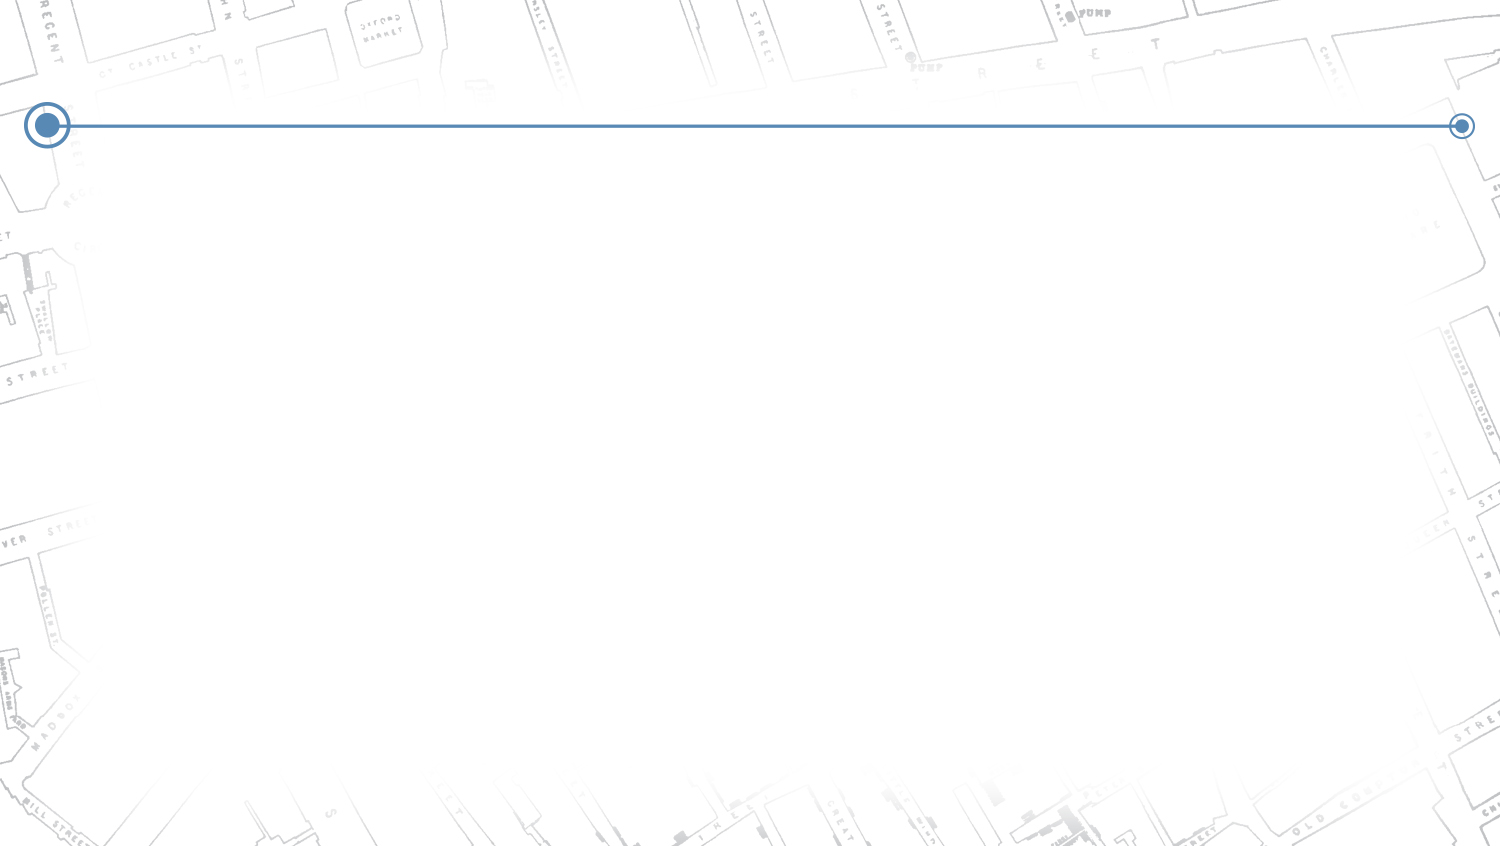
\includegraphics[height=\paperheight,width=\paperwidth]{Template/slides/Basic1.jpg}}
\setbeamertemplate{frametitle}
{\begin{flushright}\vspace{.23in}{\insertframetitle\hspace{.2in}}\end{flushright}}
\setbeamertemplate{footline}{%
\leavevmode%
  \hbox{%
    \begin{beamercolorbox}[wd=\paperwidth,ht=2.5ex,dp=1.125ex]{palette quaternary}%
    \vspace{.08in}\insertnavigation{\paperwidth}{}{\hskip0pt plus1filll}
    \end{beamercolorbox}%
  }
}
}
\makeatother

% Basic2

\makeatletter
\define@key{beamerframe}{Basic2}[true]{%
\usebackgroundtemplate{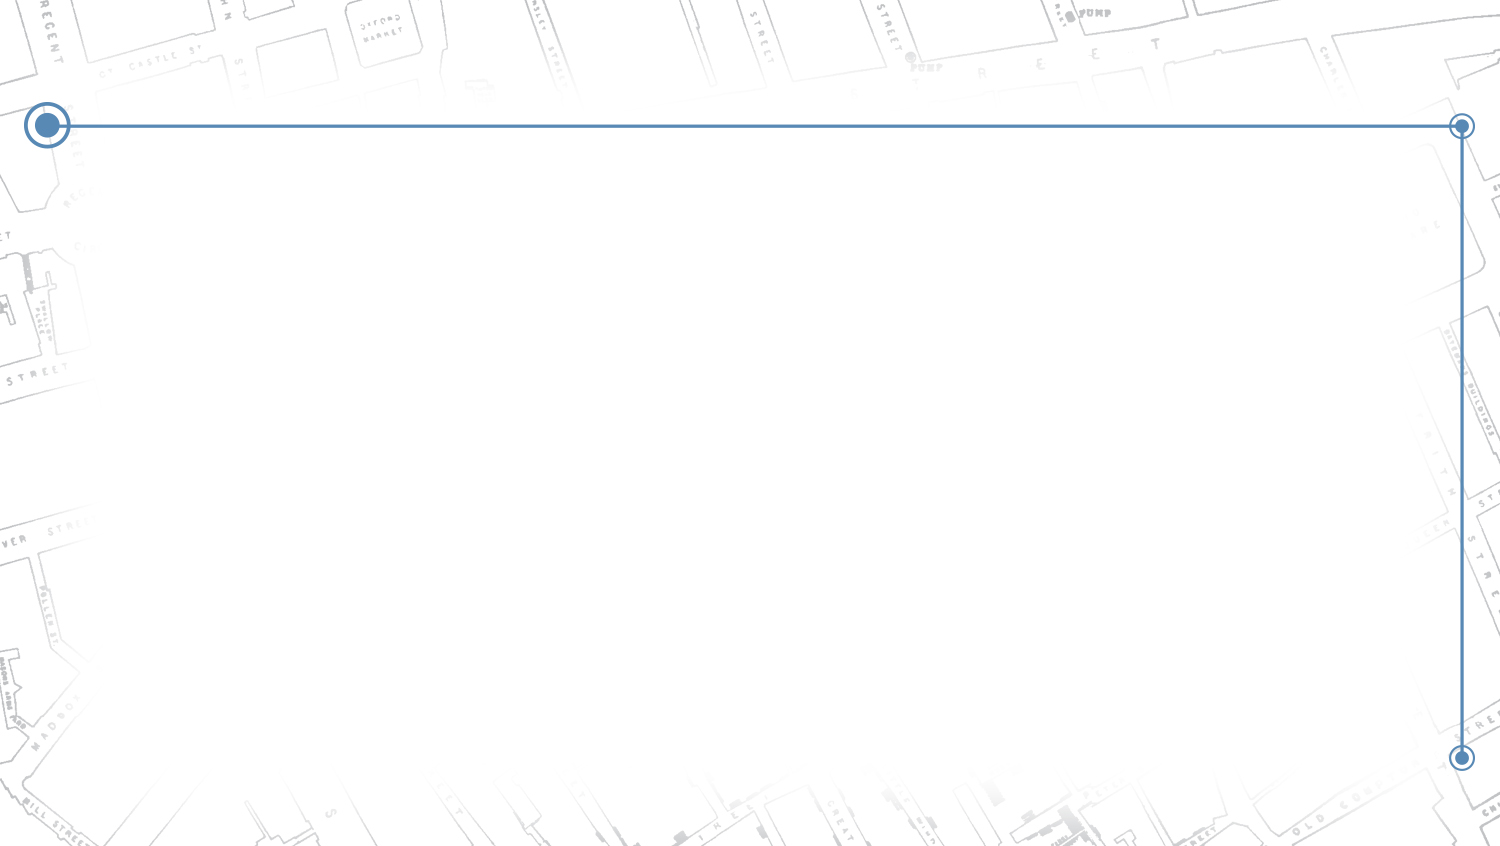
\includegraphics[height=\paperheight,width=\paperwidth]{Template/slides/Basic2.jpg}}
\setbeamertemplate{frametitle}
{\begin{flushright}\vspace{.23in}{\insertframetitle\hspace{.2in}}\end{flushright}}
\setbeamertemplate{footline}{%
\leavevmode%
  \hbox{%
    \begin{beamercolorbox}[wd=\paperwidth,ht=2.5ex,dp=1.125ex]{palette quaternary}%
    \vspace{.08in}\insertnavigation{\paperwidth}{}{\hskip0pt plus1filll}
    \end{beamercolorbox}%
  }
}
}
\makeatother

% Basic3

\makeatletter
\define@key{beamerframe}{Basic3}[true]{%
\usebackgroundtemplate{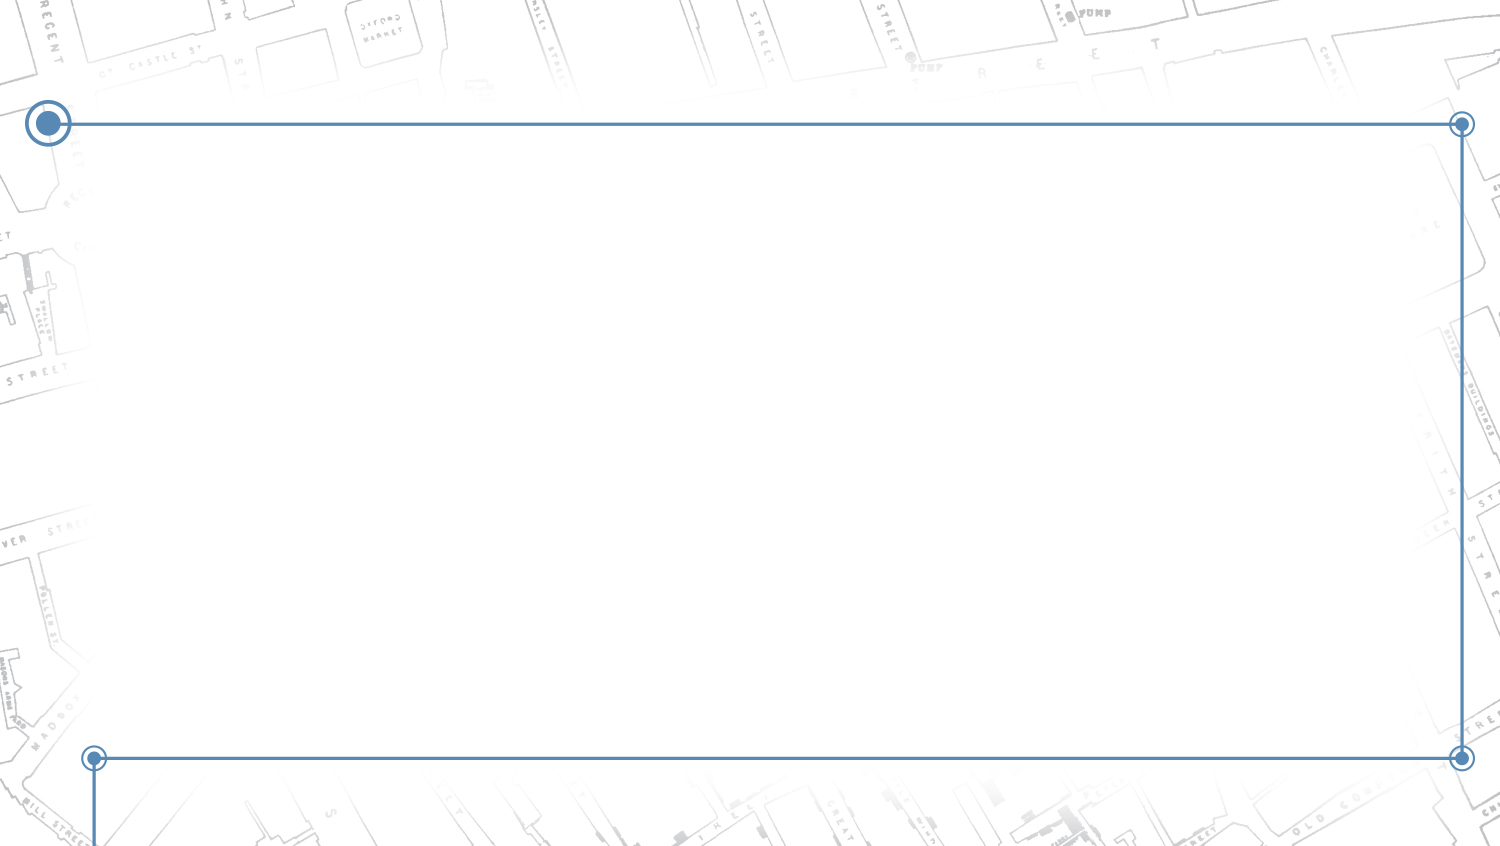
\includegraphics[height=\paperheight,width=\paperwidth]{Template/slides/Basic3.jpg}}
\setbeamertemplate{frametitle}
{\begin{flushright}\vspace{.23in}{\insertframetitle\hspace{.2in}}\end{flushright}}
\setbeamertemplate{footline}{}
}
\makeatother

% Basic1Logo

\makeatletter
\define@key{beamerframe}{Basic1Logo}[true]{%
\usebackgroundtemplate{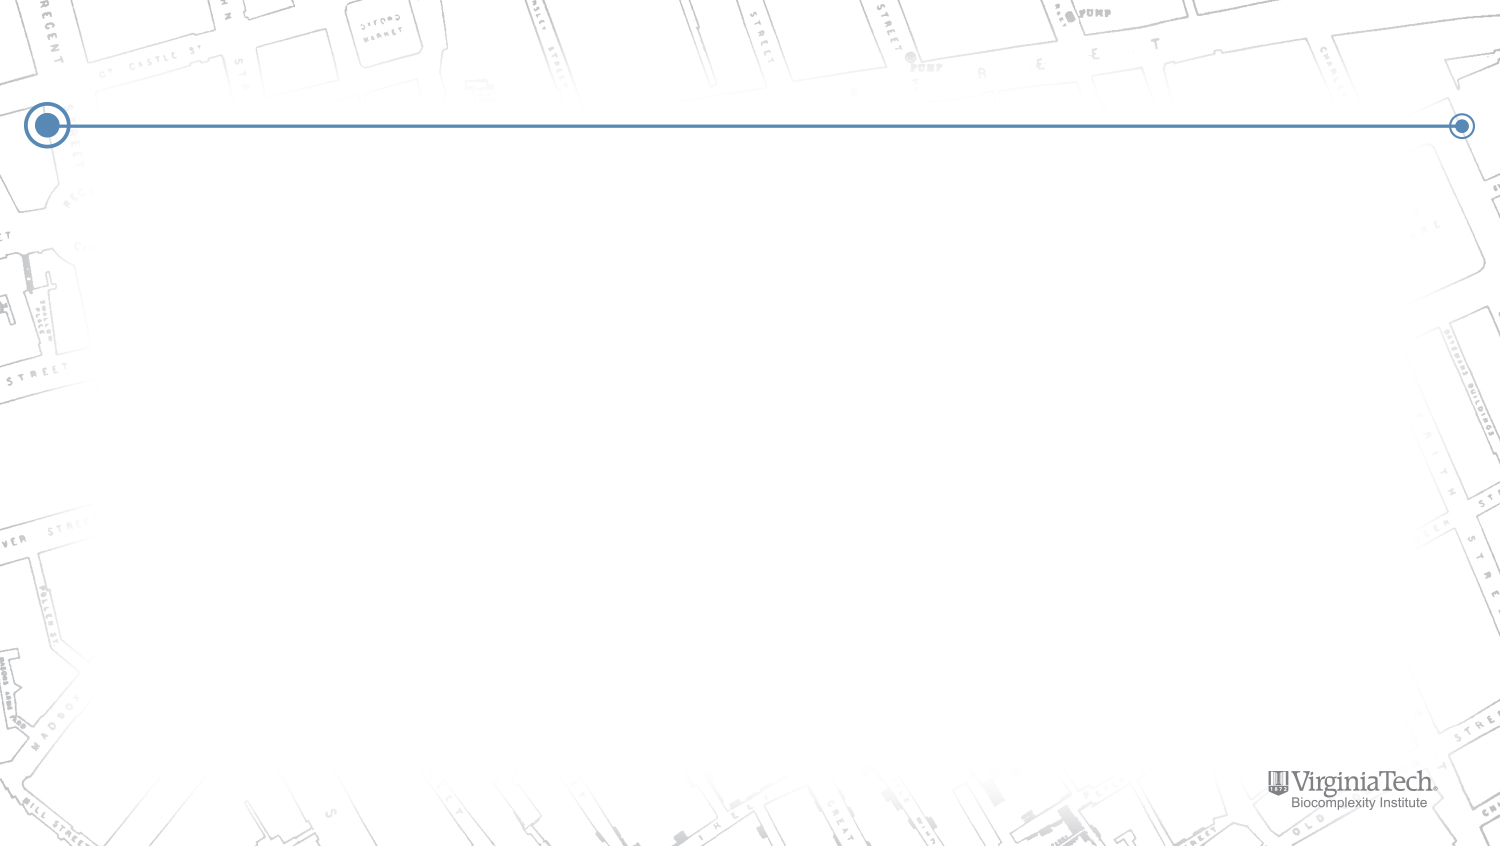
\includegraphics[height=\paperheight,width=\paperwidth]{Template/slides/Basic1Logo.jpg}}
\setbeamertemplate{frametitle}
{\begin{flushright}\vspace{.23in}{\insertframetitle\hspace{.2in}}\end{flushright}}
\setbeamertemplate{footline}{}
}
\makeatother

% Basic2Logo

\makeatletter
\define@key{beamerframe}{Basic2Logo}[true]{%
\usebackgroundtemplate{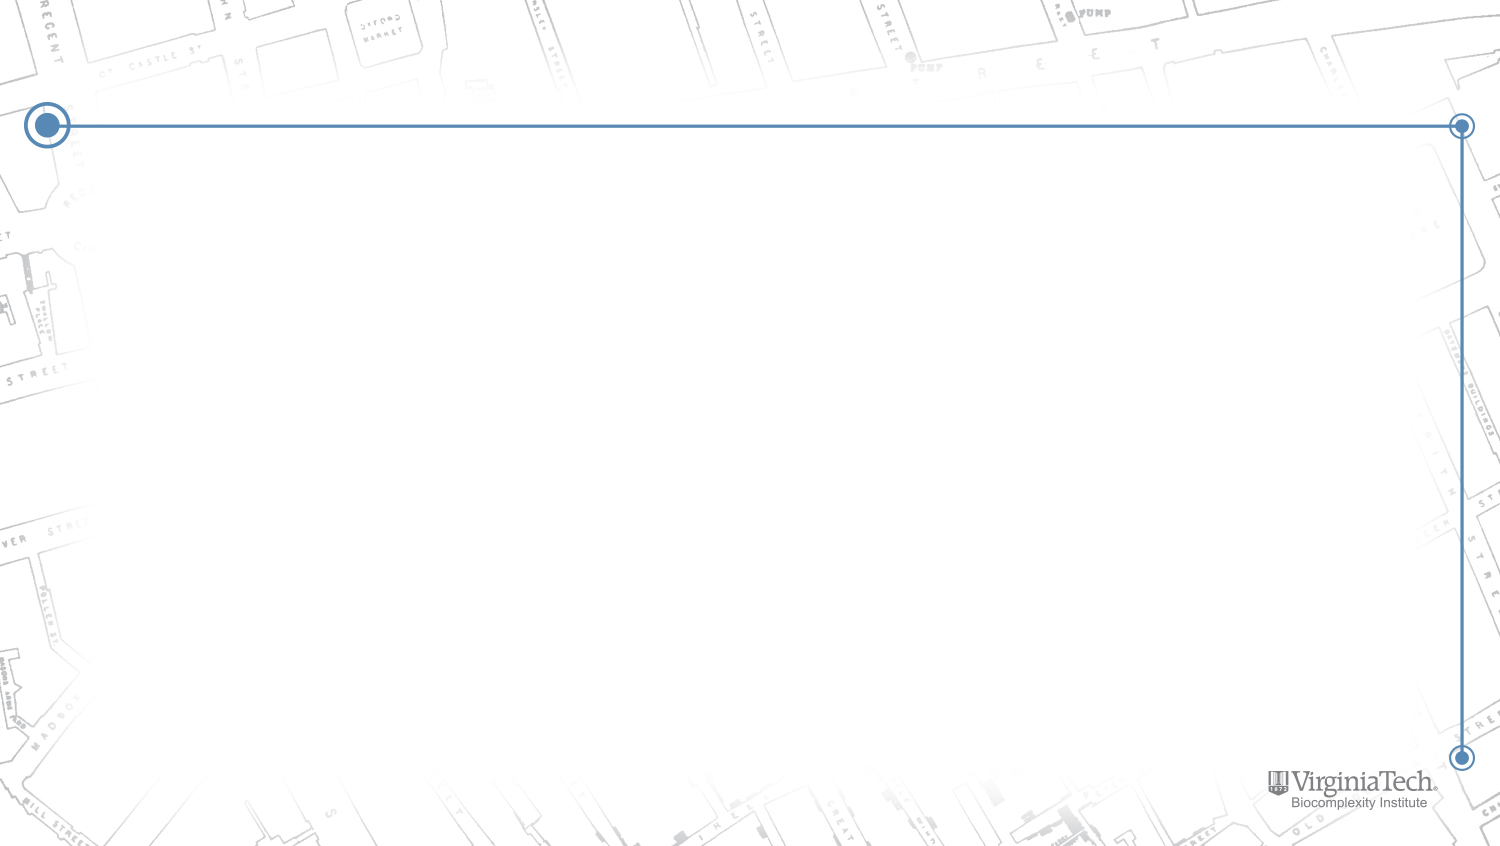
\includegraphics[height=\paperheight,width=\paperwidth]{Template/slides/Basic2Logo.jpg}}
\setbeamertemplate{frametitle}
{\begin{flushright}\vspace{.23in}{\insertframetitle\hspace{.2in}}\end{flushright}}
\setbeamertemplate{footline}{}
}
\makeatother

% Basic3Logo

\makeatletter
\define@key{beamerframe}{Basic3Logo}[true]{%
\usebackgroundtemplate{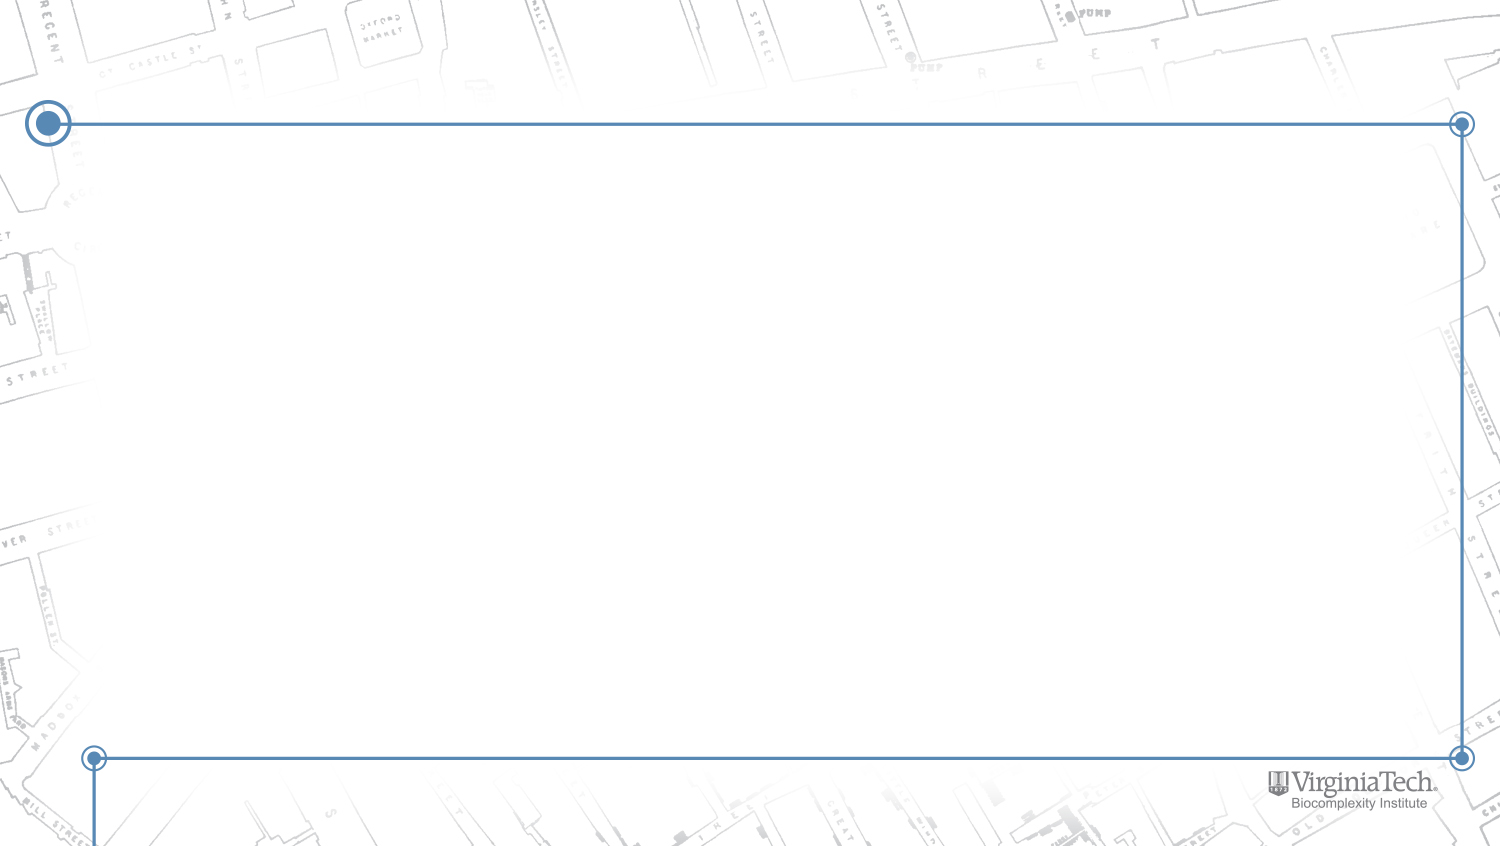
\includegraphics[height=\paperheight,width=\paperwidth]{Template/slides/Basic3Logo.jpg}}
\setbeamertemplate{frametitle}
{\begin{flushright}\vspace{.23in}{\insertframetitle\hspace{.2in}}\end{flushright}}
\setbeamertemplate{footline}{}
}
\makeatother

% Section

\makeatletter
\define@key{beamerframe}{Section}[true]{%
%\setbeamertemplate{frametitle}[default][right]
%\addtobeamertemplate{frametitle}{\vskip1.4in\hspace*{-.7in}}{}
\usebackgroundtemplate{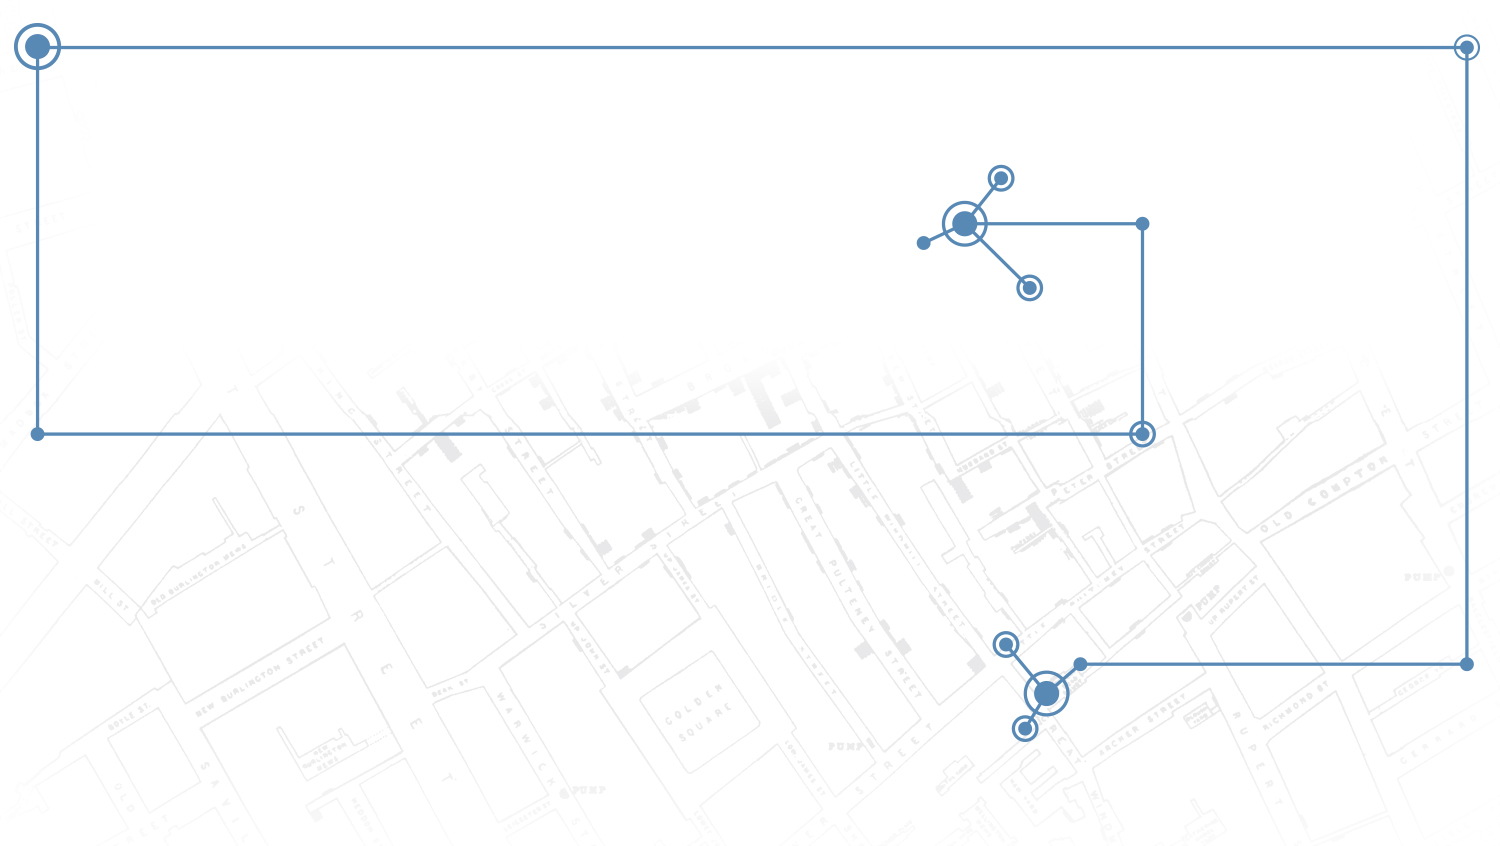
\includegraphics[height=\paperheight,width=\paperwidth]{Template/slides/Section.jpg}}
\hspace*{-1.8in}
\setbeamertemplate{frametitle}
{\begin{flushright}\vskip1.5in{\insertframetitle}\end{flushright}}
\setbeamertemplate{footline}{}
}
\makeatother

\mode
<all>


% This file includes instructions on how to use the template
% e.g., how to call up specific frame formats

% The necessary packages are already loaded within the .sty document.
% You must add specific ones if needed depending on your needs.

%%%%%%%%%%%%%%%%%%%%%%%%%%%%%%
%%%%%%%%%%%%%%%%%%%%%%%%%%%%%%

\documentclass[compress]{beamer}
\ProvidesPackageRCS $Header: SDAL_Beamer.sty ,v 1 05/13/2016 $

\mode<presentation>

% Set presentation size

\usepackage[orientation=landscape,size=custom,width=16,height=9,scale=0.5,debug]{beamerposter} 
\setbeamersize{text margin left=.25in,text margin right=.25in}

% Set Fonts

%\usepackage[T1]{fontenc}
%\usepackage[default]{raleway}
 
 \usefonttheme{serif}
 
 \setbeamerfont{frametitle}{series=\bfseries} 
\setbeamerfont{title}{series=\bfseries} 
\setbeamerfont{author}{series=\bfseries} 

%\usepackage[T1]{fontenc}
%\usepackage[nosfdefault]{raleway}

% Set the size of the font

\usepackage{scrextend}
\changefontsizes{14pt}
\setbeamerfont{title}{size=\fontsize{17pt}{17pt}}
\setbeamerfont{author}{size=\fontsize{14pt}{14pt}}
\setbeamerfont{frametitle}{size=\fontsize{17pt}{17pt}}
\setbeamerfont{date}{size=\fontsize{14pt}{14pt}}
\setbeamerfont*{structure}{size*={17pt}{17pt}}
\setbeamerfont*{tiny structure}{size*={6pt}{6pt}}
  
% Table of Contents

\setbeamertemplate{section in toc}[ball]
\setbeamertemplate{subsection in toc}[square]

\setbeamertemplate{subsection in toc}{\hspace{1.2em}{\color{BIlightblue}\rule[0.3ex]{6pt}{6pt}}~\inserttocsubsection\par}

% Set Color

\definecolor{VTmaroon}{RGB}{102,0,0} 
\definecolor{VTorange}{RGB}{255,102,0}
\definecolor{BIdarkblue}{RGB}{18,37,45}
\definecolor{BIaquablue}{RGB}{126,168,173}
\definecolor{BIcoolgrey}{RGB}{153,153,153}
\definecolor{BIlightblue}{RGB}{93,137,180}
\definecolor{BIlightgreen}{RGB}{141,194,136}

 
\setbeamercolor*{title}{fg=black}
\setbeamercolor{author}{fg=black} 
\setbeamercolor{frametitle}{fg=black} 
\setbeamercolor{section in toc}{fg=black}
\setbeamercolor{subsection in toc}{fg=black}
\setbeamercolor{itemize subsubitem}{fg=black}
\setbeamercolor{itemize subitem}{fg=black}
\setbeamercolor{itemize item}{fg=black}
\setbeamercolor{section number projected}{bg=BIlightblue,fg=white}

% Lists

\makeatletter
\renewcommand{\itemize}[1][]{%
  \beamer@ifempty{#1}{}{\def\beamer@defaultospec{#1}}%
  \ifnum \@itemdepth >2\relax\@toodeep\else
    \advance\@itemdepth\@ne
    \beamer@computepref\@itemdepth% sets \beameritemnestingprefix
    \usebeamerfont{itemize/enumerate \beameritemnestingprefix body}%
    \usebeamercolor[fg]{itemize/enumerate \beameritemnestingprefix body}%
    \usebeamertemplate{itemize/enumerate \beameritemnestingprefix body begin}%
    \list
      {\usebeamertemplate{itemize \beameritemnestingprefix item}}
      {%
        \setlength\topsep{0pt}%NEW
        \setlength\partopsep{0pt}%NEW
        \setlength\itemsep{0pt}%NEW
        \def\makelabel##1{%
          {%
            \hss\llap{{%
                \usebeamerfont*{itemize \beameritemnestingprefix item}%
                \usebeamercolor[fg]{itemize \beameritemnestingprefix item}##1}}%
          }%
        }%
      }
  \fi%
  \beamer@cramped%
  \raggedright%
  \beamer@firstlineitemizeunskip%
}
\makeatother

\setlength\topsep{-10pt}
\setlength\partopsep{-10pt}


\setbeamertemplate{itemize items}[circle]
\setbeamertemplate{itemize subitem}{---}
\setbeamertemplate{itemize subsubitem}[circle]

% TOC

\makeatletter
\patchcmd{\beamer@sectionintoc}
  {\vfill}
  {\vskip\itemsep}
  {}
  {}
\makeatother  

% Remove navigation symbols

\setbeamertemplate{navigation symbols}{}

% Format Title Page

\defbeamertemplate*{title page}{customized}[1][]
{
\centering
\vspace{.9in}\hspace*{-3.8in}
\begin{overlayarea}{4.1in}{1cm}
\centering{
\usebeamerfont{title}\inserttitle\par}
\usebeamerfont{subtitle}\usebeamercolor[fg]{subtitle}\insertsubtitle\par
\end{overlayarea}\\
\vspace{.2in}\hspace*{-1in}
\begin{overlayarea}{4in}{1cm}
\centering{
\usebeamerfont{date}\insertdate\par \vspace{.1in}
\usebeamerfont{author}\insertauthor\par
\usebeamerfont{institute}\insertinstitute\par}
\end{overlayarea}
}

%%% Formatting Different Frame Styles

% Title

\makeatletter
\define@key{beamerframe}{Title}[true]{%
\usebackgroundtemplate{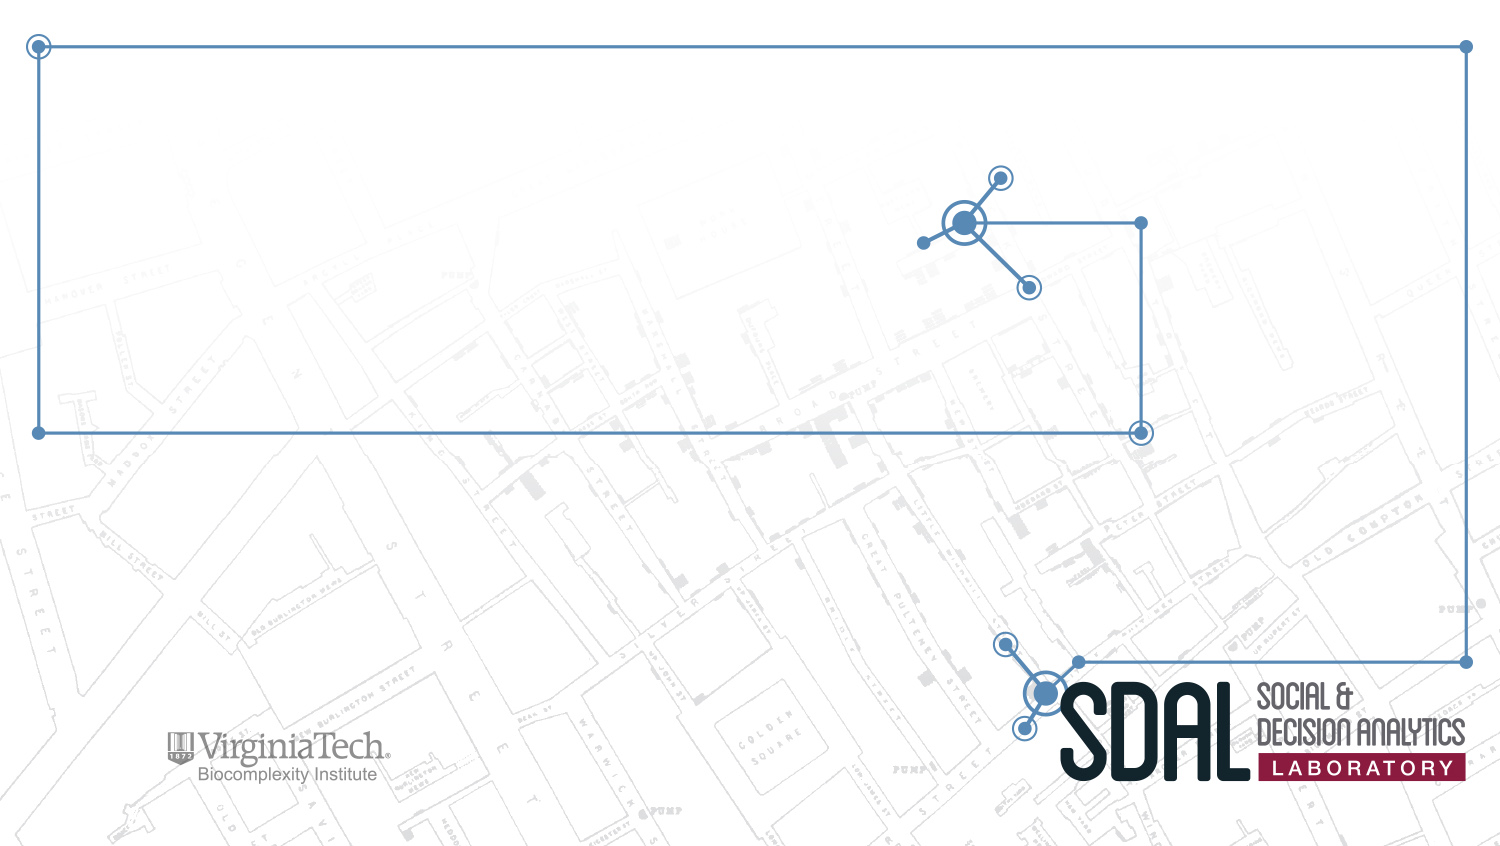
\includegraphics[height=\paperheight,width=\paperwidth]{Template/slides/Title.jpg}
\setbeamertemplate{frametitle}[default][right]
\addtobeamertemplate{frametitle}{\vskip.1in\hspace*{.5in}}{}}
\setbeamertemplate{footline}{}
}
\makeatother

% Outline

\makeatletter
\define@key{beamerframe}{ToC}[true]{%
\usebackgroundtemplate{
\includegraphics[height=\paperheight,width=\paperwidth]{Template/slides/Blank.jpg}}
\setbeamertemplate{frametitle}[default][right]
\addtobeamertemplate{frametitle}{\vskip.1in\hspace*{.5in}}{}
\setbeamertemplate{footline}{}
}
\makeatother

% Blank

\makeatletter
\define@key{beamerframe}{Blank}[true]{%
\usebackgroundtemplate{
\includegraphics[height=\paperheight,width=\paperwidth]{Template/slides/Blank.jpg}}
\setbeamertemplate{frametitle}
{\begin{flushright}\vspace{.23in}{\insertframetitle\hspace{.2in}}\end{flushright}}
\setbeamertemplate{footline}{%
\leavevmode%
  \hbox{%
    \begin{beamercolorbox}[wd=\paperwidth,ht=2.5ex,dp=1.125ex]{palette quaternary}%
    \vspace{.08in}\insertnavigation{\paperwidth}{}{\hskip0pt plus1filll}
    \end{beamercolorbox}%
  }
}
}
\makeatother

% BlankLogo

\makeatletter
\define@key{beamerframe}{BlankLogo}[true]{%
\usebackgroundtemplate{
\includegraphics[height=\paperheight,width=\paperwidth]{Template/slides/BlankLogo.jpg}}
\setbeamertemplate{frametitle}
{\begin{flushright}\vspace{.23in}{\insertframetitle\hspace{.2in}}\end{flushright}}
\setbeamertemplate{footline}{}
}
\makeatother

% Basic1

\makeatletter
\define@key{beamerframe}{Basic1}[true]{%
\usebackgroundtemplate{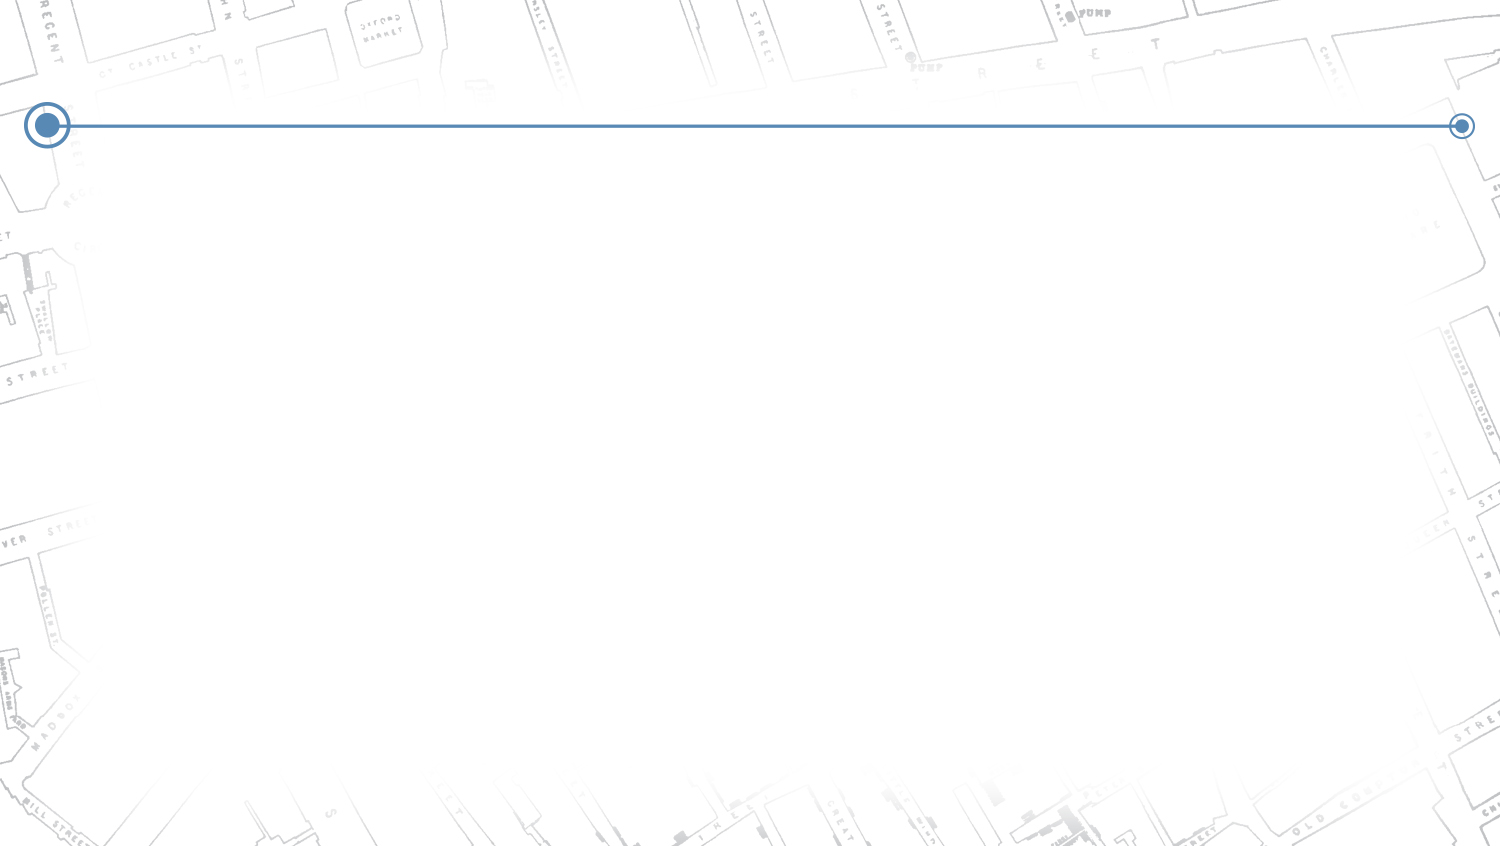
\includegraphics[height=\paperheight,width=\paperwidth]{Template/slides/Basic1.jpg}}
\setbeamertemplate{frametitle}
{\begin{flushright}\vspace{.23in}{\insertframetitle\hspace{.2in}}\end{flushright}}
\setbeamertemplate{footline}{%
\leavevmode%
  \hbox{%
    \begin{beamercolorbox}[wd=\paperwidth,ht=2.5ex,dp=1.125ex]{palette quaternary}%
    \vspace{.08in}\insertnavigation{\paperwidth}{}{\hskip0pt plus1filll}
    \end{beamercolorbox}%
  }
}
}
\makeatother

% Basic2

\makeatletter
\define@key{beamerframe}{Basic2}[true]{%
\usebackgroundtemplate{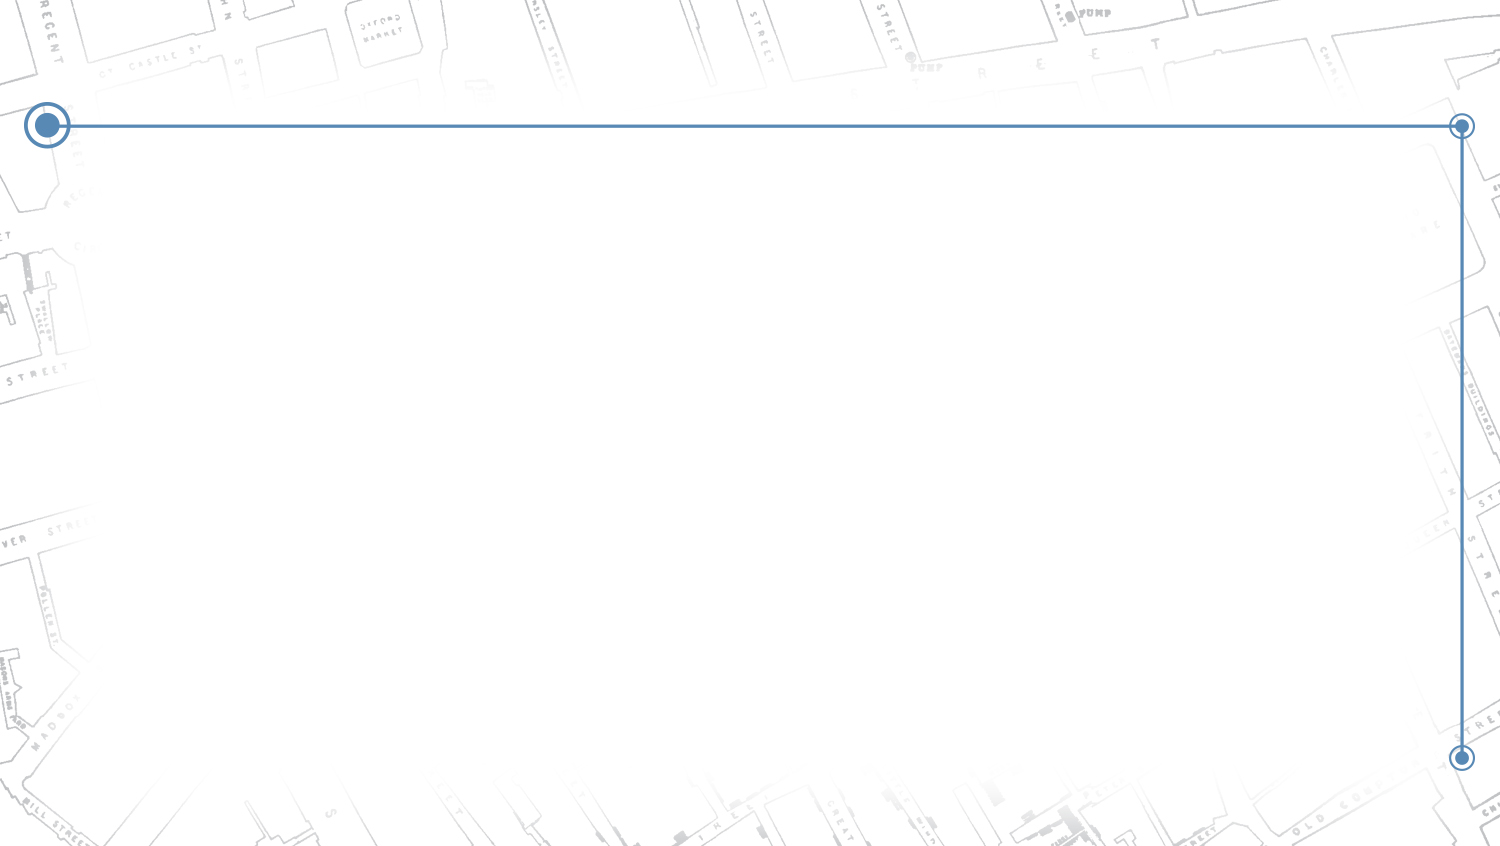
\includegraphics[height=\paperheight,width=\paperwidth]{Template/slides/Basic2.jpg}}
\setbeamertemplate{frametitle}
{\begin{flushright}\vspace{.23in}{\insertframetitle\hspace{.2in}}\end{flushright}}
\setbeamertemplate{footline}{%
\leavevmode%
  \hbox{%
    \begin{beamercolorbox}[wd=\paperwidth,ht=2.5ex,dp=1.125ex]{palette quaternary}%
    \vspace{.08in}\insertnavigation{\paperwidth}{}{\hskip0pt plus1filll}
    \end{beamercolorbox}%
  }
}
}
\makeatother

% Basic3

\makeatletter
\define@key{beamerframe}{Basic3}[true]{%
\usebackgroundtemplate{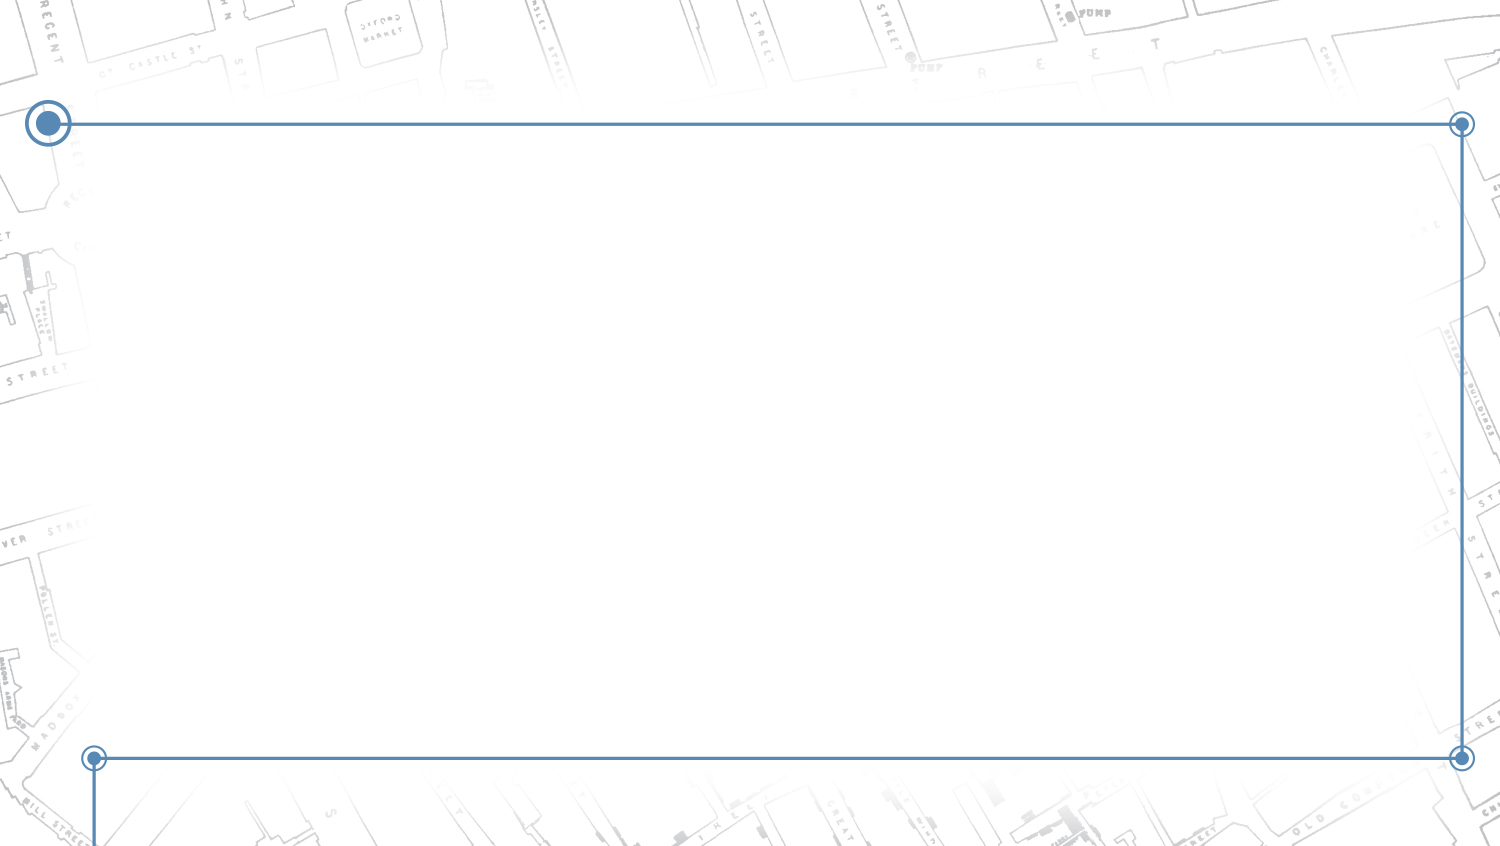
\includegraphics[height=\paperheight,width=\paperwidth]{Template/slides/Basic3.jpg}}
\setbeamertemplate{frametitle}
{\begin{flushright}\vspace{.23in}{\insertframetitle\hspace{.2in}}\end{flushright}}
\setbeamertemplate{footline}{}
}
\makeatother

% Basic1Logo

\makeatletter
\define@key{beamerframe}{Basic1Logo}[true]{%
\usebackgroundtemplate{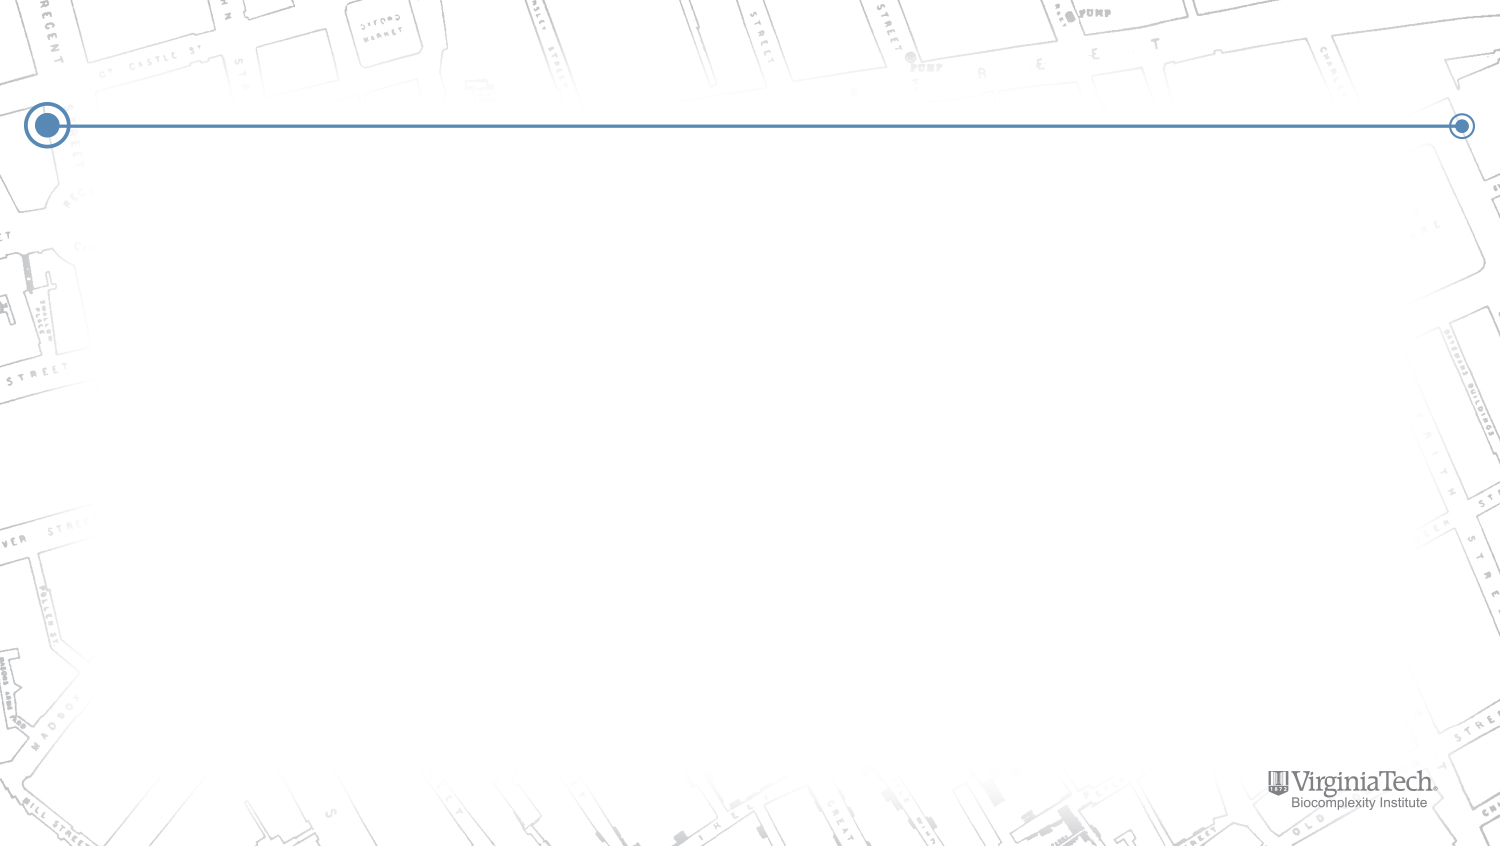
\includegraphics[height=\paperheight,width=\paperwidth]{Template/slides/Basic1Logo.jpg}}
\setbeamertemplate{frametitle}
{\begin{flushright}\vspace{.23in}{\insertframetitle\hspace{.2in}}\end{flushright}}
\setbeamertemplate{footline}{}
}
\makeatother

% Basic2Logo

\makeatletter
\define@key{beamerframe}{Basic2Logo}[true]{%
\usebackgroundtemplate{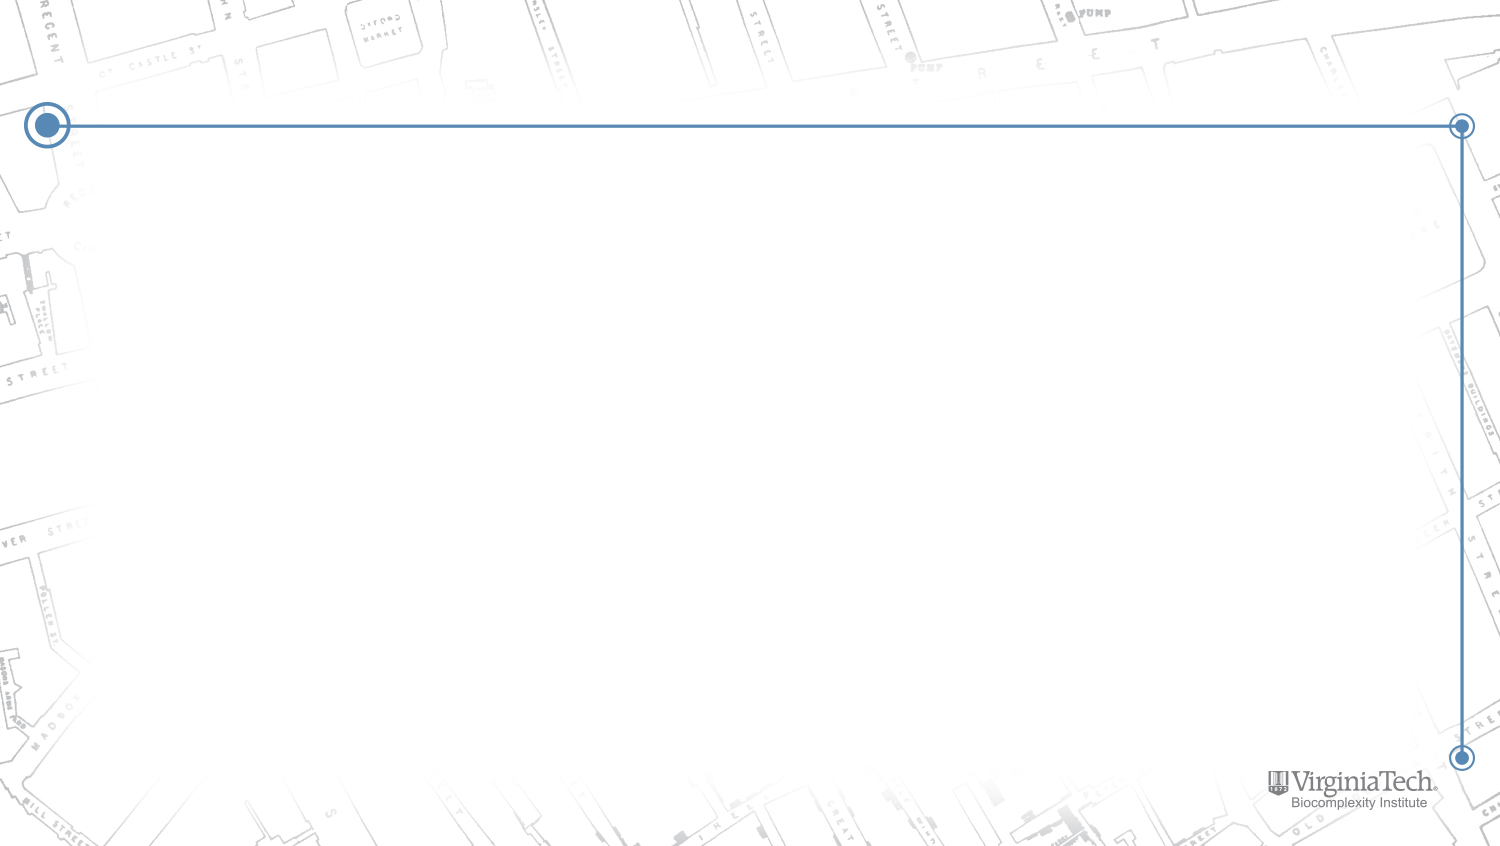
\includegraphics[height=\paperheight,width=\paperwidth]{Template/slides/Basic2Logo.jpg}}
\setbeamertemplate{frametitle}
{\begin{flushright}\vspace{.23in}{\insertframetitle\hspace{.2in}}\end{flushright}}
\setbeamertemplate{footline}{}
}
\makeatother

% Basic3Logo

\makeatletter
\define@key{beamerframe}{Basic3Logo}[true]{%
\usebackgroundtemplate{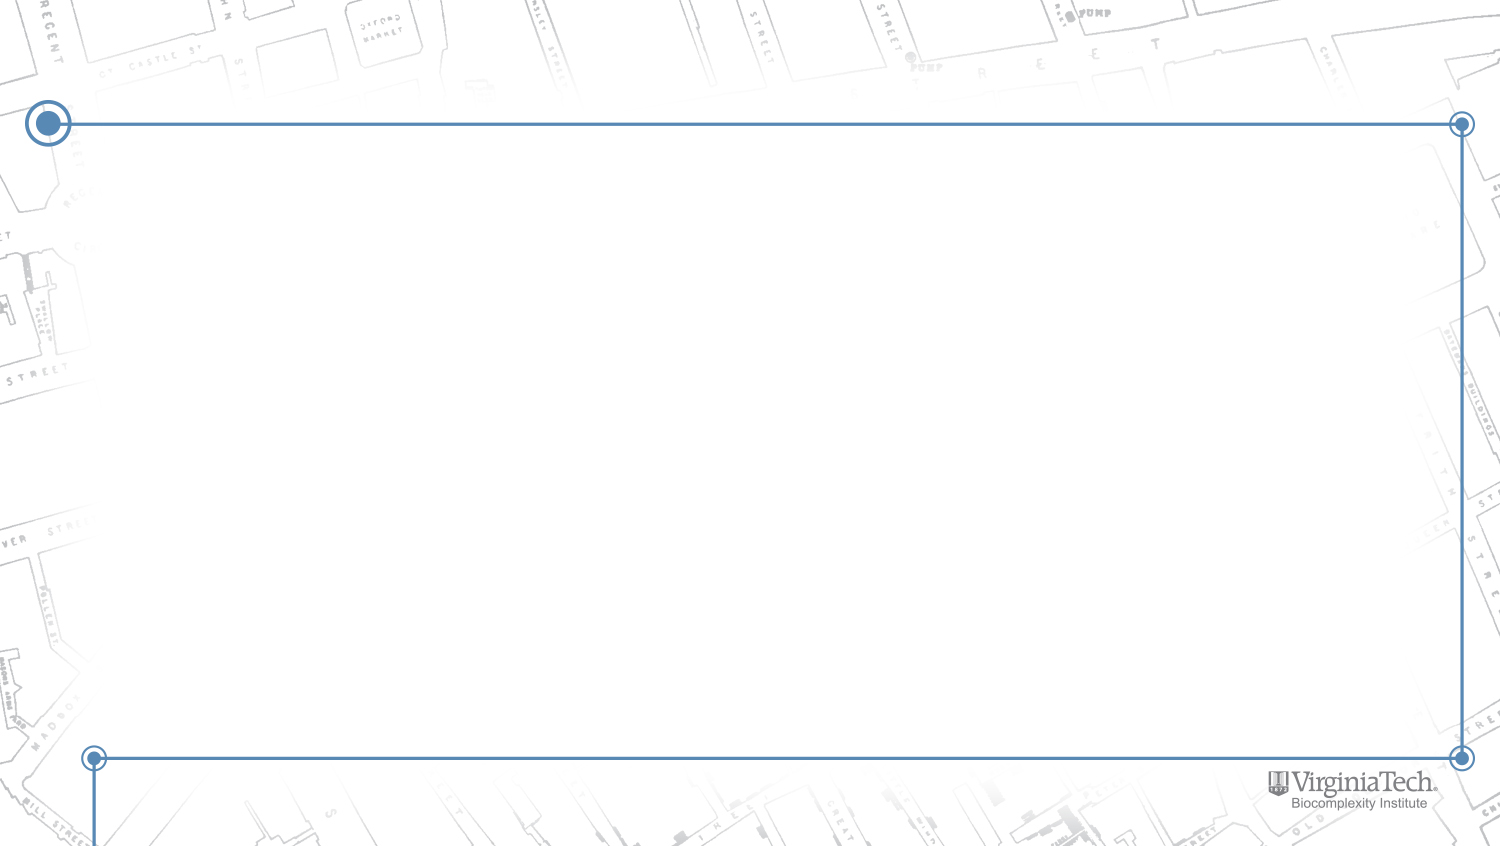
\includegraphics[height=\paperheight,width=\paperwidth]{Template/slides/Basic3Logo.jpg}}
\setbeamertemplate{frametitle}
{\begin{flushright}\vspace{.23in}{\insertframetitle\hspace{.2in}}\end{flushright}}
\setbeamertemplate{footline}{}
}
\makeatother

% Section

\makeatletter
\define@key{beamerframe}{Section}[true]{%
%\setbeamertemplate{frametitle}[default][right]
%\addtobeamertemplate{frametitle}{\vskip1.4in\hspace*{-.7in}}{}
\usebackgroundtemplate{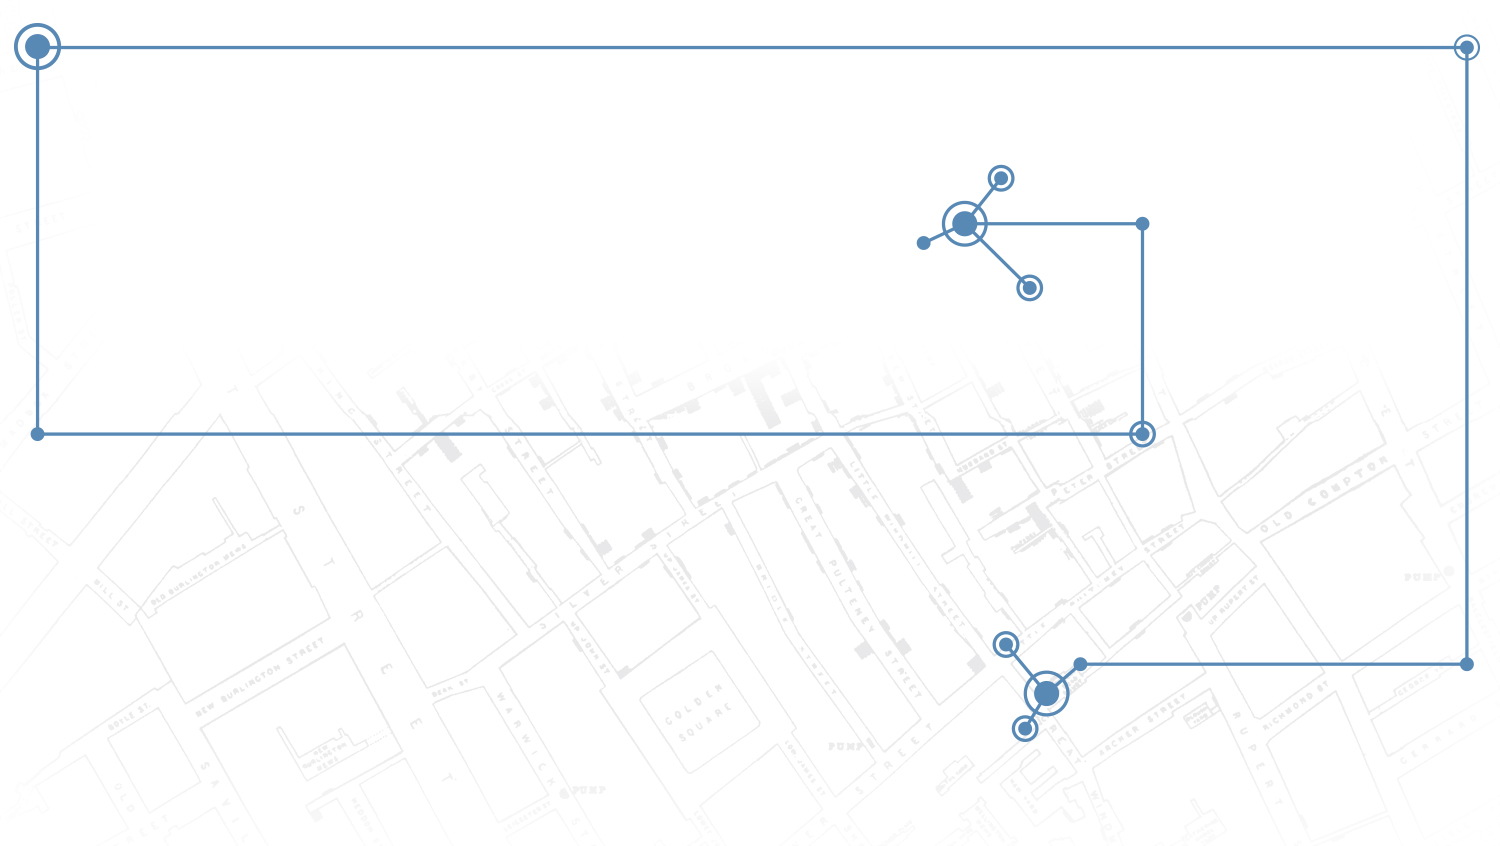
\includegraphics[height=\paperheight,width=\paperwidth]{Template/slides/Section.jpg}}
\hspace*{-1.8in}
\setbeamertemplate{frametitle}
{\begin{flushright}\vskip1.5in{\insertframetitle}\end{flushright}}
\setbeamertemplate{footline}{}
}
\makeatother

\mode
<all>


\usepackage[english]{babel}

\usepackage{csquotes}

\usepackage[pscoord]{eso-pic}% The zero point of the coordinate systemis the lower left corner of the page (the default).

\newcommand{\placetextbox}[3]{% \placetextbox{<horizontal pos>}{<vertical pos>}{<stuff>}
    \setbox0=\hbox{#3}% Put <stuff> in a box
    \AddToShipoutPictureFG*{% Add <stuff> to current page foreground
        \put(\LenToUnit{#1\paperwidth},\LenToUnit{#2\paperheight}){\vtop{{\null}\makebox[0pt][c]{#3}}}%
    }%
}%

\usepackage{caption}
\captionsetup[figure]{labelformat=empty}% redefines the caption setup of the figures environment in the beamer class.


% Template Colors: VTmaroon, VTorange, BIdarkblue, BIaquablue, BIcoolgrey, BIlightblue, BIlightgreen

\title[SDAL]{\vspace{-0.85in}Changing People's Minds: Understanding Social Diffusion Dynamics Using Networked Cognitive Systems}
\author{Daniel Chen, MPH\\ \tiny{Computational. Network. Epidemiology.}}
\date[]{September 1, 2016}

% For long titles and/or subtitles, will need to use \vspace[-XXin] to align accordingly

\begin{document}

    \begin{frame}[BlankLogo] \frametitle{}
        \begin{figure}
    \centering
    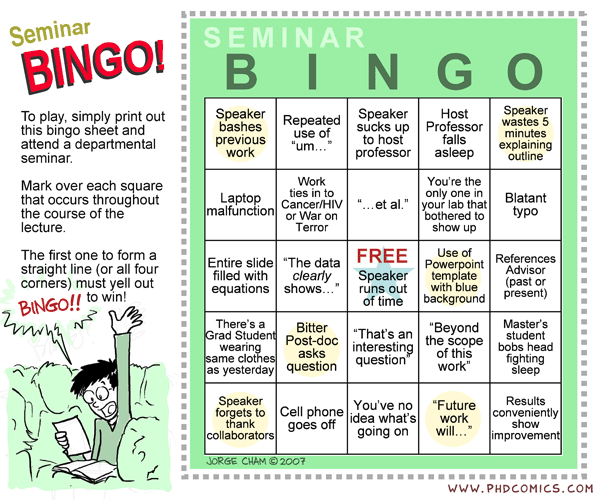
\includegraphics[height=0.9\textheight]{../phd040907s_bingo}
    \label{fig:phd040907sbingo}
    \end{figure}

    \end{frame}

    \begin{frame}[Title]
        \titlepage
    \end{frame}

% If you do not want an outline, do not include this slide
% Edit toc depth for what level you want included

%    \begin{frame}[ToC] \frametitle{Outline}
%    \setcounter{tocdepth}{2}
%    \hfill
%    \parbox[t]{.95\textwidth}{
%        \begin{minipage}[c][0.75\textheight]{\textwidth}
%            \linespread{1}
%            \tableofcontents
%        \end{minipage}
%    }
%    \end{frame}

% Note on progress tracker:
% If you do not want the progress tracker in the footer, do not use \section or \subsections
% Progress tracker online works on Blank, Basic 1 and Basic 2 slide types

% Compile twice after adding sections and subsection to get them to appear
% Subsections are represented by the dots in the footer. Do not use sections if you do not want the dots.
% Place subsections right above that slide to have dots highlight appropriately

\section[SDAL]{SDAL}

    \begin{frame}[Section] \frametitle{\vspace{-0.2in}Social \& Decision Analytics\\Laboratory}
    \end{frame}

\subsection[Social and Decision Analytics Laboratory (SDAL)]{Social and Decision Analytics Laboratory (SDAL)}

    \begin{frame}[Basic2] \frametitle{The Social and Decision Analytics Laboratory}
        Founded in 2013
        \vspace{3mm}

        \begin{columns}
            \begin{column}{0.5\textwidth}
                \begin{figure}
                    \centering
                    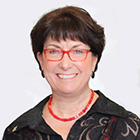
\includegraphics[width=2cm]{../figures/keller-sallie-140-w}
                    \caption{Sallie Keller\\Director\\Professor}
                    \label{fig:keller-sallie-140-w}
                \end{figure}
            \end{column}
            \begin{column}{0.5\textwidth}  %%<--- here
                \begin{figure}
                    \centering
                    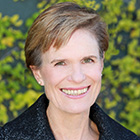
\includegraphics[width=2cm]{../figures/shipp-stephanie-140-w}
                        \caption{Stephanie Shipp\\Deputy Director\\Research Professor}
                    \label{fig:shipp-stephanie-140-w}
                \end{figure}
            \end{column}
        \end{columns}

        \begin{displayquote}
        statisticians and social and behavioral scientists to embrace today’s data revolution, developing evidence-based research and quantitative methods to inform policy decision-making.
        \end{displayquote}
    \end{frame}

\subsection[SDAL II]{SDAL II}
    \begin{frame}[Basic2] \frametitle{The Social and Decision Analytics Laboratory}
        \begin{figure}
            \centering
            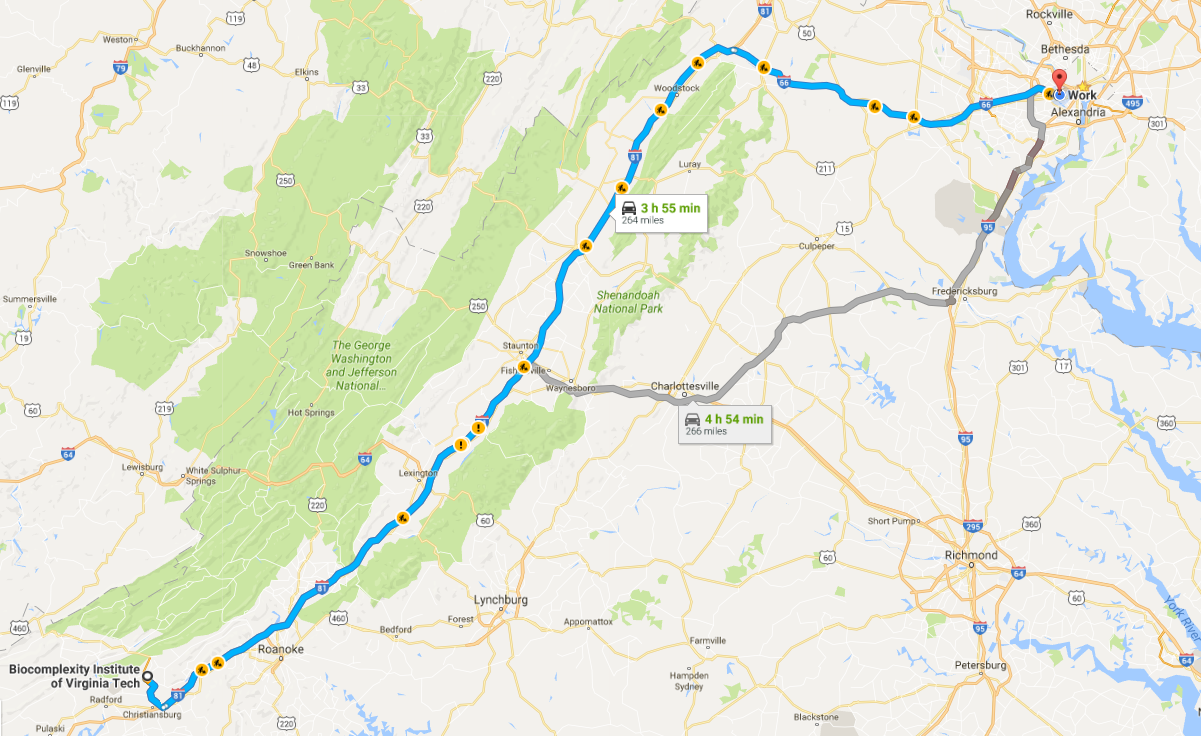
\includegraphics[height=0.75\textheight]{../figures/sdal_google_maps}
            \label{fig:sdalgooglemaps}
        \end{figure}
    \end{frame}

    \begin{frame}[Blank] \frametitle{People}
        \small
        \begin{columns}
            \begin{column}{0.3\textwidth}
                \textbf{Research Faculty}
                \begin{enumerate}
                    \item David Higdon (Statistics)
                    \item Viki Lancaster (Statistics)
                    \item Mark Orr (Psychology)
                    \item Aaron Schroeder (Data Science)
                    \item Gizem Korkmaz (Economics)
                \end{enumerate}
            \end{column}

            \begin{column}{0.3\textwidth}
                \textbf{Post Doctoral Associates}
                \begin{enumerate}
                    \item Kathryn Ziemer (Psychology)
                    \item Bianica Pires (Social Science)
                    \item Emily Molfino (Political Science)
                    \item Joshua Goldstein (Statistics)
                \end{enumerate}

                \textbf{Visiting Scholars \& Collaborators:} 7
            \end{column}

            \begin{column}{0.3\textwidth}
                \textbf{Students}
                \begin{enumerate}
                    \item Daniel Chen (GRA: GBCB)
                    \item Adrienne Rogers (VT: Statistics)
                    \item Emily Stark (Austin Peay: Mathematics)
                \end{enumerate}

                \textbf{Administrative Staff}
                \begin{enumerate}
                    \item Kimberly Lyman
                    \item Tracie Hase
                \end{enumerate}
            \end{column}
        \end{columns}
    \end{frame}

\subsection[Projects]{Projects}

    \begin{frame}[Basic2] \frametitle{Projects}
        \begin{enumerate}
            \item Assessing New Data Sources for the Federal Census
            \item Simulating Urban Air Pollution Exposure
            \item Collaborating to Build a Culture of Health
            \item Leveraging Data to Enhance Emergency Response
            \item Practicing Data Science for the Public Good
            \item Modeling the Spread of Beliefs Through Social Media
        \end{enumerate}

    \end{frame}

\subsection[Data Science for the Public Good]{Data Science for the Public Good}

    \begin{frame}[Basic2] \frametitle{Data Science for the Public Good}

        \begin{columns}
            \begin{column}{0.5\textwidth}
                \begin{itemize}
                    \item First summer for the The Data Science for the Public Good program (DSPG)
                    \item Research Experience for Undergraduates (REU) funded by NSF
                    \item Bash, SSH, \LaTeX, R, SQL, GIS, Literate Programming, Web Scraping, Git
                \end{itemize}
            \end{column}
            \begin{column}{0.5\textwidth}
                \begin{figure}
                    \centering
                    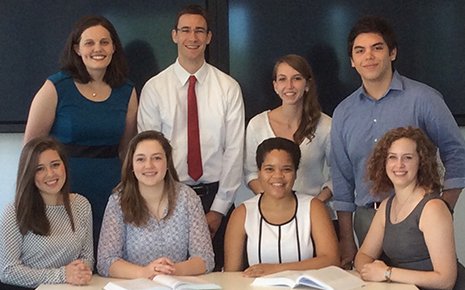
\includegraphics[width=0.9\linewidth]{../figures/data-science-for-public-good-student-photo-overview}
                    \caption{My Students! :D}
                    \label{fig:data-science-for-public-good-student-photo-overview}
                \end{figure}
            \end{column}
        \end{columns}
    \end{frame}

\subsection[Come Visit]{Come Visit}

    \begin{frame}[Blank] \frametitle{Come Visit!}
        \begin{columns}
            \begin{column}{0.35\textwidth}
                \begin{figure}
                    \centering
                    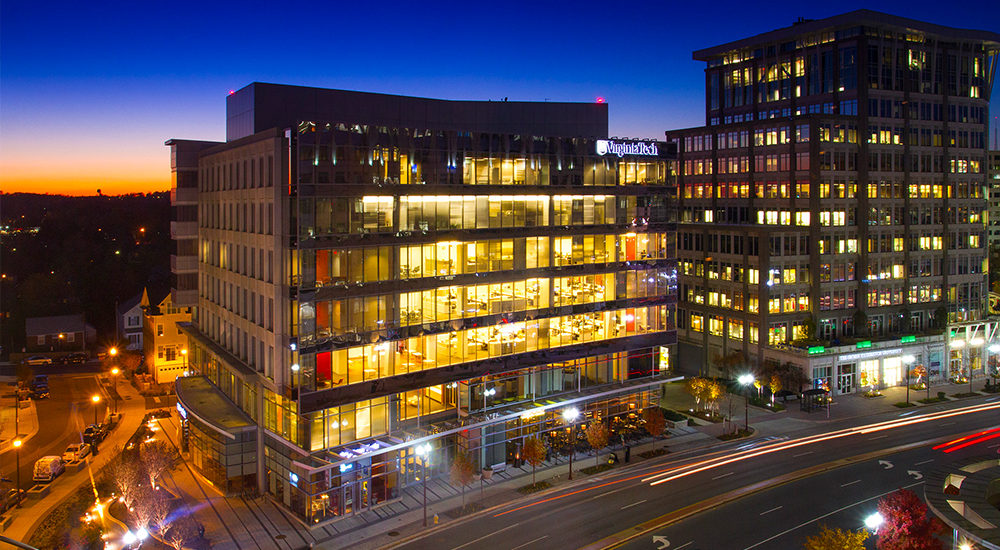
\includegraphics[width=1\linewidth]{../figures/metro-lab-big-data-sdal-header}
                    \caption{}
                    \label{fig:metro-lab-big-data-sdal-header}
                \end{figure}

                \begin{figure}
                    \centering
                    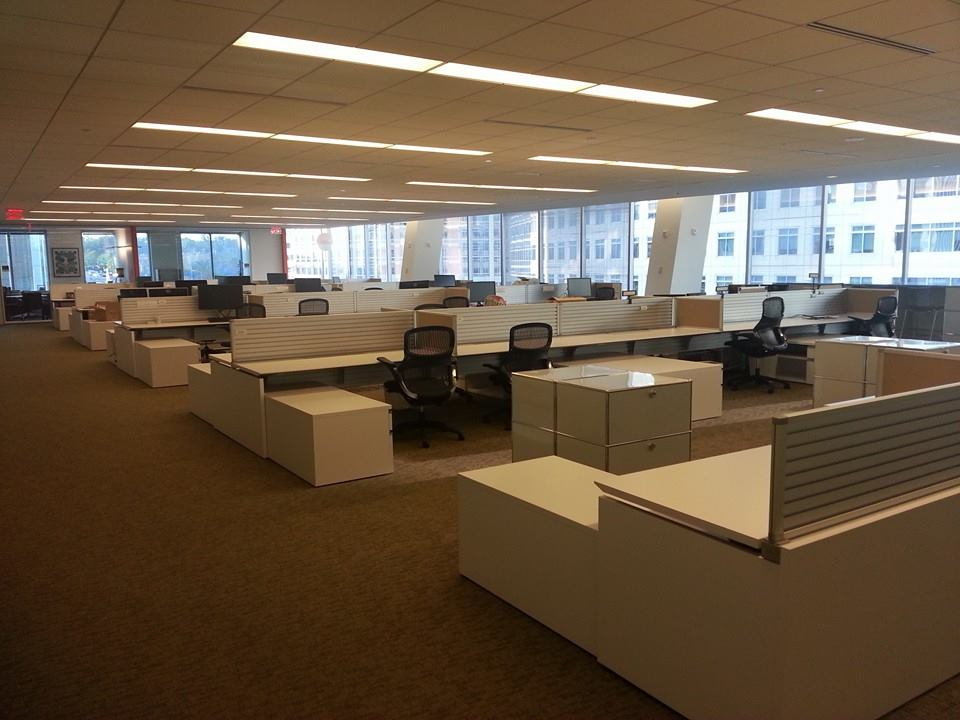
\includegraphics[width=1\linewidth]{../figures/sdal_pit}
                    \caption{}
                    \label{fig:sdalpit}
                \end{figure}
            \end{column}

            \begin{column}{0.65\textwidth}
                \begin{figure}
                    \centering
                    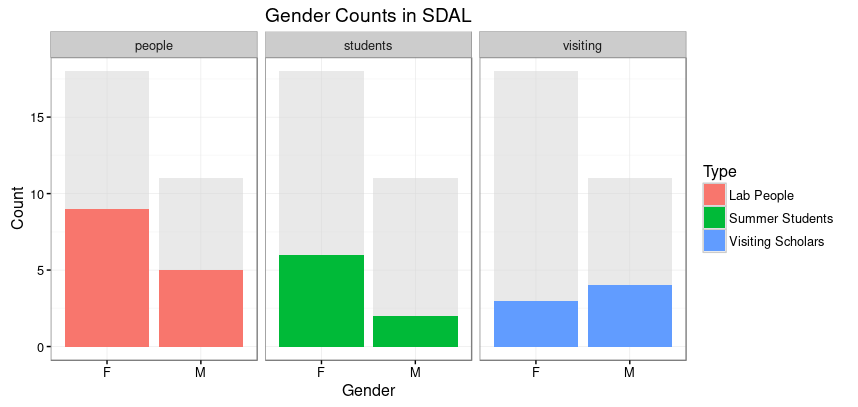
\includegraphics[width=1.0\linewidth]{../figures/sdal_gender_breakdown}
                    \caption{}
                    \label{fig:sdalgenderbreakdown}
                    \end{figure}
            \end{column}
        \end{columns}
    \end{frame}

\section[Introduction]{Introduction}

    \begin{frame}[Section] \frametitle{\vspace{-0.2in}Modeling the Spread of Beliefs\\Through Social Media}
    \end{frame}

\subsection[Epidemiology]{Epidemiology}

    \begin{frame}[Basic2] \frametitle{Epidemiology}
        \begin{columns}
            \begin{column}{0.5\textwidth}
                \begin{displayquote}
                    Epidemiology is the science of population health,
                    aiming to \textbf{understand} the key causes of health and disease and
                    doing so in a way that it may inform \textbf{interventions} so we may act
                \end{displayquote}
            \end{column}
            \begin{column}{0.5\textwidth}
                $\vcenter{\centering
\includegraphics[width=0.5\linewidth]{../figures/epi-matters}}$
            \end{column}
        \end{columns}
    \end{frame}

\subsection[Epidemiology II]{Epidemiology II}
    \begin{frame}[Basic2] \frametitle{Epidemiology}
        \begin{itemize}
            \item Infectious Diseases (Ebola, Zika, Measles, etc)
            \item \textbf{Chronic Diseases} (diabetes, obesity, smoking, etc)
        \end{itemize}
    \end{frame}

\subsection[Epidemiology III]{Epidemiology III}
    \begin{frame}[Basic2] \frametitle{Columbia MPH Certificates $\sim$ GBCB}
        \begin{columns}
            \begin{column}{0.5\textwidth}
                \begin{itemize}
                    \tiny
                    \item \textbf{Advanced Epidemiology}
                    \item \textbf{Applied Biostatistics}
                    \item Child, Youth, and Family Health
                    \item Climate and Health
                    \item \textbf{Comparative Effectiveness Outcomes Research}
                    \item Environmental Health Policy
                    \item \textbf{Epidemiology of Chronic Disease}
                    \item Global Health
                    \item Health and Human Rights
                    \item Health of an Aging Society
                    \item Health Policy Analysis
                    \item Health Policy and Practice
                \end{itemize}
            \end{column}
            \begin{column}{0.5\textwidth}
                \begin{itemize}
                    \tiny
                    \item Health Promotion Research and Practice
                    \item History, Ethics, and Law
                    \item \textbf{Infectious Disease Epidemiology}
                    \item \textbf{Injury Prevention and Control}
                    \item Molecular Epidemiology
                    \item Public Health and Humanitarian Assistance
                    \item \textbf{Public Health Informatics}
                    \item \textbf{Public Health Research Methods}
                    \item Sexuality, Sexual and Reproductive Health
                    \item \textbf{Social Determinants of Health}
                    \item Toxicology
                \end{itemize}
            \end{column}
        \end{columns}
    \end{frame}

\subsection{Modeling}
    \begin{frame}[Basic2] \frametitle{(Computational) (Infectious) Disease Modeling}
        Two main types of models:
        \begin{enumerate}
            \item Compartmental/Mathematical/System Dynamics/\\
                Ordinary Differential Equation (ODE) Models
            \item Agent-Based Models (ABM)
        \end{enumerate}
    \end{frame}

\subsection{Compartmental Models I}
    \begin{frame}[Basic2] \frametitle{Compartmental Models}
        \begin{columns}
            \begin{column}{0.4\textwidth}
                \vspace{2mm}

                \textbf{SIR Models}
                \begin{itemize}
                    \item \textbf{S}usceptible
                    \item \textbf{I}nfectious
                    \item \textbf{R}ecovered
                \end{itemize}
                \vspace{-1mm}
                \begin{align*}
                    \frac{dS}{dt} &= -b S(t) I(t)\\
                    \frac{dI}{dt} &= b S(t) I(t) - kI(t)\\
                    \frac{dR}{dt} &= k I(t)
                \end{align*}
            \end{column}

            \begin{column}{0.6\textwidth}
                
                \vspace{2mm}
                
                \begin{figure}
                    \centering
                    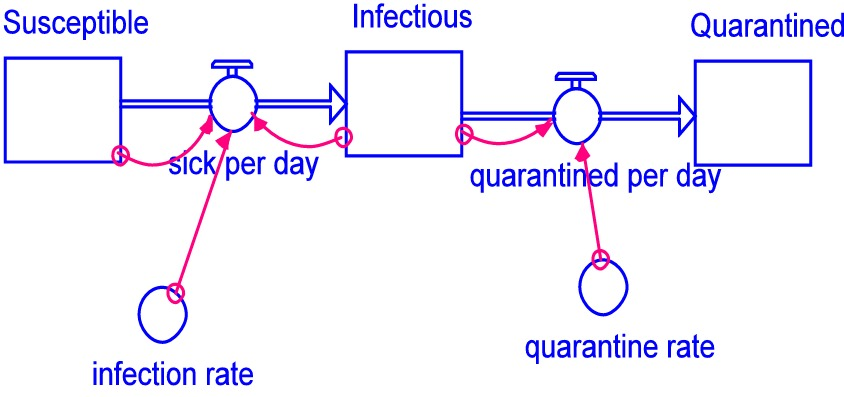
\includegraphics[width=0.90\linewidth]{../figures/stella-sir}
                    \caption{Example SIR model from Stella\\(Maryland Virtual High School)}
                    \label{fig:stella-sir}
                \end{figure}

            \end{column}
        \end{columns}
    \end{frame}

\subsection{Compartmental Models II}
    \begin{frame}[Basic2] \frametitle{Compartmental Models}
        \begin{columns}
            \begin{column}{0.4\textwidth}
                
                \begin{itemize}
                    \item SIS
                    \item SEIR
                    \item MSIR
                    \item SI(CR)
                    \item Vaccine
                \end{itemize}
            \end{column}
            \begin{column}{0.6\textwidth}
                \vspace{2mm}
                
                Pros
                \begin{itemize}
                    \item Deterministic
                    \item Overall System Dynamics
                    \item Homogeneous (random mixing)
                    \item Simple, easy to set up
                \end{itemize}
                Cons
                \begin{itemize}
                    \item Not stochastic
                    \item No individual level behaviors
                    \item No complex interactions
                \end{itemize}
            \end{column}
        \end{columns}
    \end{frame}

\subsection{Agent-Based Models}

    \begin{frame}[Basic2] \frametitle{Agent-Based Models}
        \begin{columns}
            \begin{column}{0.5\textwidth}
                \begin{itemize}
                    \item The model is composed of individual `agents'
                    \item Each agent has a set of rules
                    \item The agents repeat these rules (ticks/cycles)
                \end{itemize}
            \end{column}
            \begin{column}{0.5\textwidth}
                Observe complex system dynamics from the bottom-up through \textbf{emergence}
            \end{column}
        \end{columns}
    \end{frame}

\subsection{Agent-Based Models Examples I}

    \begin{frame}[Blank] \frametitle{ABM Examples}
        \begin{columns}
            \begin{column}{0.5\textwidth}
                \begin{figure}
                    \centering
                    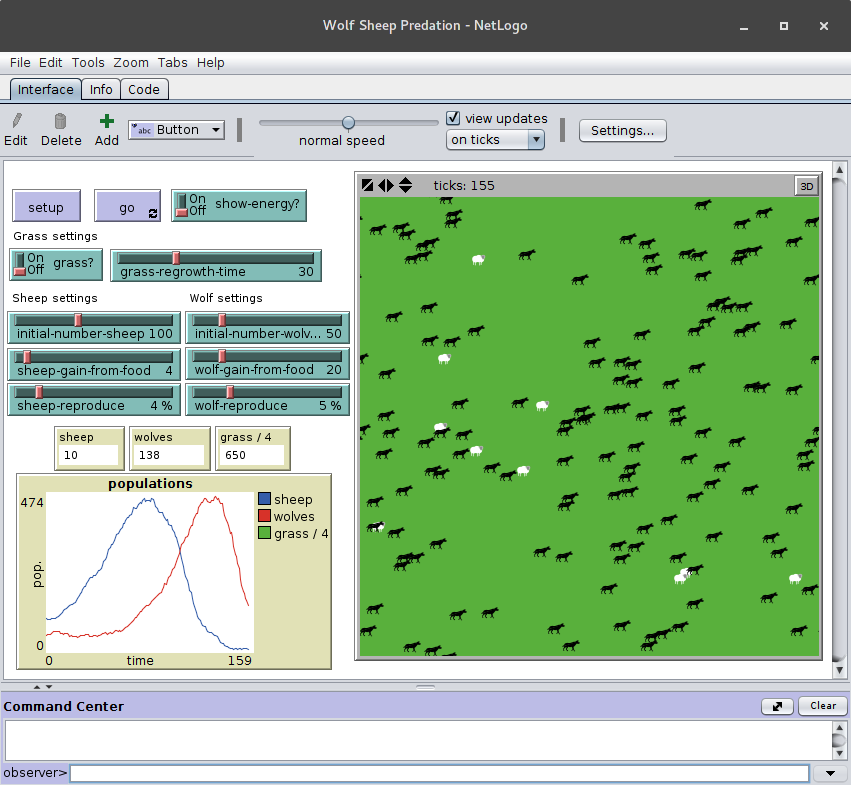
\includegraphics[width=1.0\linewidth]{../figures/netlogo_wolf_sheep_predation}
                    \caption{Netlogo Wolf Sheep Predation Model}
                    \label{fig:netlogowolfsheeppredation}
                \end{figure}
            \end{column}
            \begin{column}{0.5\textwidth}
                \begin{figure}
                    \centering
                    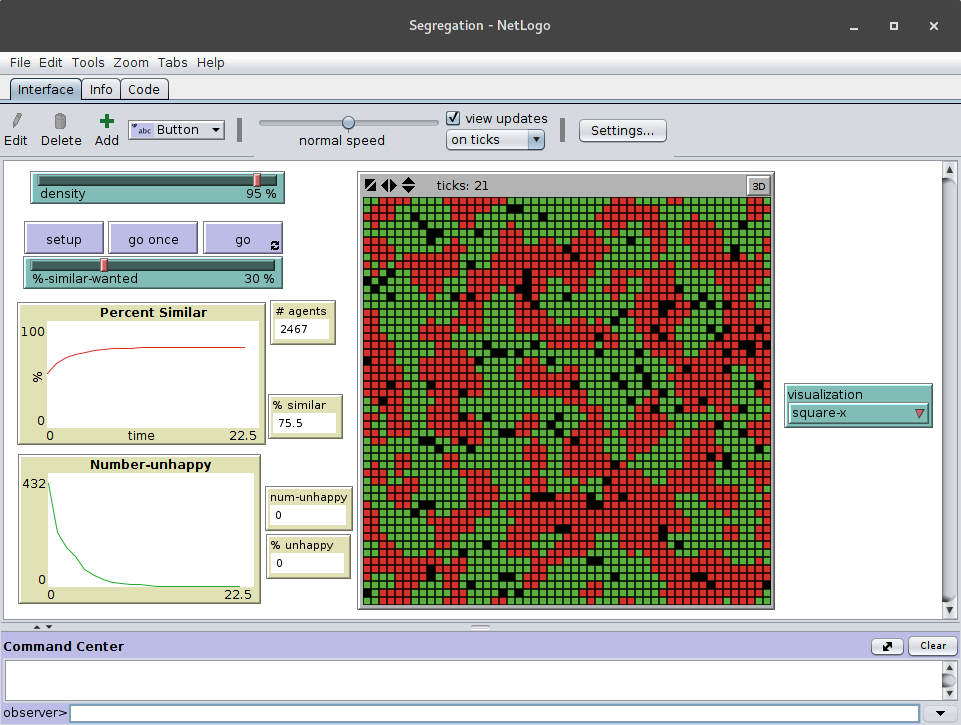
\includegraphics[width=1.0\linewidth]{../figures/netlogo_segregation}
                    \caption{Netlogo Segregation Model}
                    \label{fig:netlogosegregation}
                \end{figure}
            \end{column}
        \end{columns}
    \end{frame}

\subsection{Agent-Based Models Examples II}

    \begin{frame}[Blank] \frametitle{Virus on a Network Model}
        \begin{columns}
            \begin{column}{0.4\textwidth}
                \begin{figure}
                    \centering
                    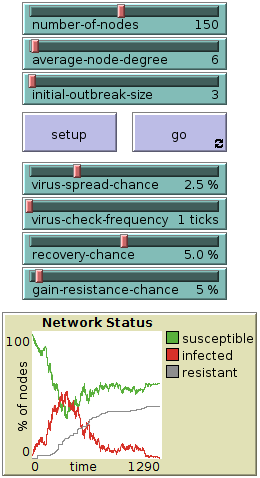
\includegraphics[height=0.85\textheight]{../figures/netlogo_virus_on_a_network_2_zoomed}
                    \caption{}
                    \label{fig:netlogovirusonanetwork2zoomed}
                \end{figure}
            \end{column}
            \begin{column}{0.6\textwidth}
                \vspace{7mm}
                \begin{figure}
                    %\centering
                    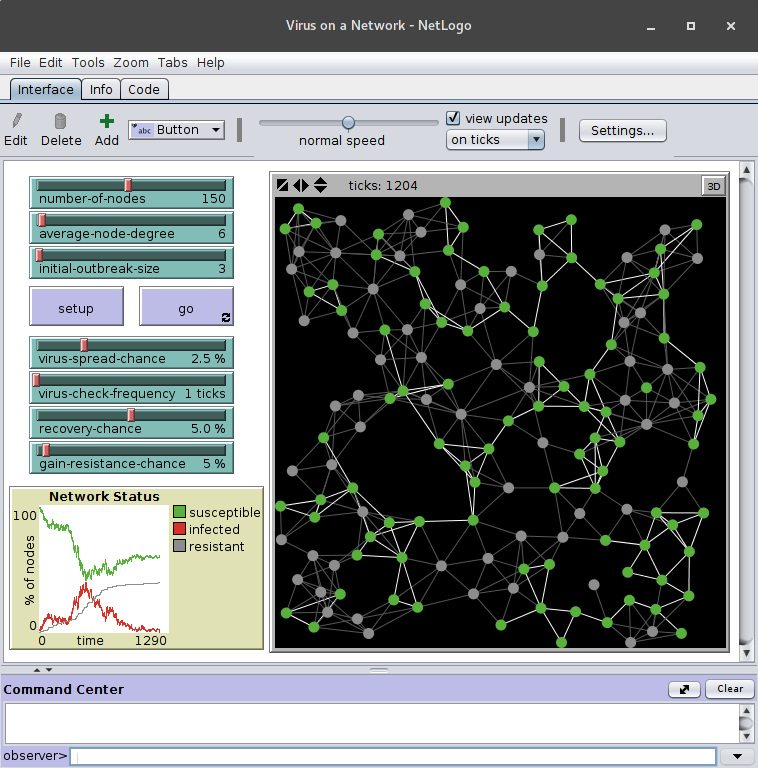
\includegraphics[width=0.77\linewidth]{../figures/netlogo_virus_on_a_network}
                    \caption{}
                    \label{fig:netlogovirusonanetwork}
                \end{figure}
            \end{column}
        \end{columns}
    \end{frame}

\subsection{Agent-Based Models II}

\begin{frame}[Basic2] \frametitle{Agent-Based Models}
    \begin{columns}
        \begin{column}{0.5\textwidth}
            Pros
            \begin{itemize}
                \item Stochastic
                \item Consolidate knowledge for agent rules/behaviors
                \item Heterogeneous
            \end{itemize}
        \end{column}
        \begin{column}{0.5\textwidth}
            Cons
            \begin{itemize}
                \item Needs a lot of data and time to set up
                \item Harder to get general system dynamics
                \item Needs a lot of model runs
                \item Resource-intensive
            \end{itemize}
        \end{column}
    \end{columns}
\end{frame}

\subsection{ABMs to CM}
    \begin{frame}[Basic2] \frametitle{ABMs to Compartmental Models}
        \begin{figure}
            \centering
            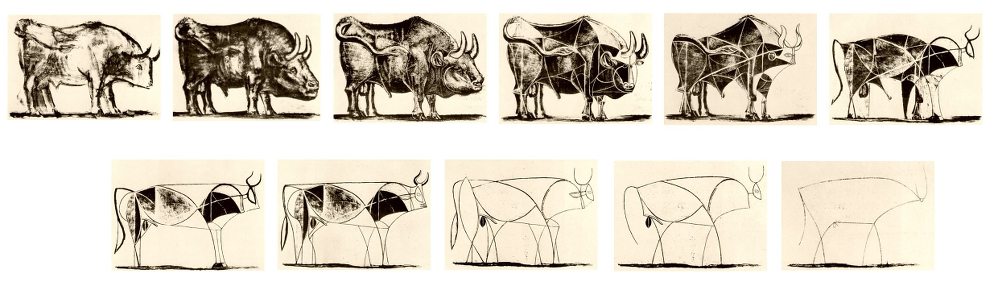
\includegraphics[width=1.0\linewidth]{../figures/Picasso-The-Bull-Lithographs-1-10}
            \caption{Pablo Picasso, ``Bull'', Plates 1-11 (Lithograph)}
            \label{fig:picasso-the-bull-lithographs-1-10}
        \end{figure}
    \end{frame}

\begin{frame}[Basic2] \frametitle{Initial Conception}
    \begin{itemize}
        \item Mark Orr, PhD.
        \item Columbia University Mailman School of Public Health
        \begin{itemize}
            \item Department of Epidemiology
            \begin{itemize}
                \item Sandro Galea, MD, MPH, DrPH
            \end{itemize}
            \item Columbia University Systems Science Program (CUSSP)
            \begin{itemize}
                \item Mailman School of Public Health (MSPH)
                \item School of Engineering and Applied Sciences (SEAS)
                \item Complex System Approaches in Population Health (CSAPH)
            \end{itemize}
        \end{itemize}
        \item Modeling obesity and attitude formation for teen sexual behaviors
    \end{itemize}
\end{frame}

\section{Watts Model}

\subsection{Duncan Watts}

    \begin{frame}[Basic2]\frametitle{Duncan Watts, PhD}
        \begin{columns}
            \begin{column}{0.4\textwidth}
                \begin{figure}
                    \centering
                    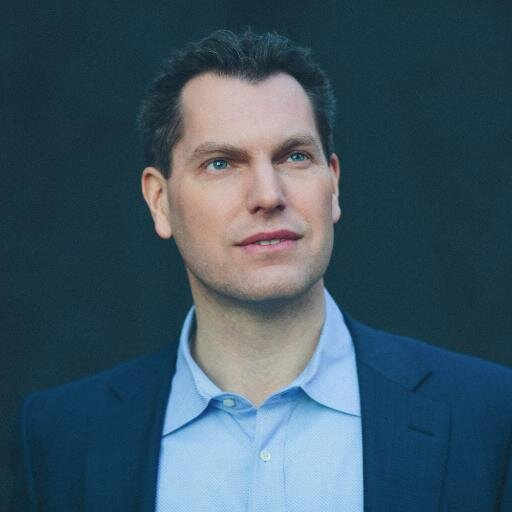
\includegraphics[width=0.8\linewidth]{../figures/watts_twitter}
                    \caption{}
                    \label{fig:wattstwitter}
                \end{figure}
            \end{column}
            \begin{column}{0.6\textwidth}
                \begin{itemize}
                    \footnotesize
                    \item Currently: Principal Researcher at Microsoft Research
                    \item Advisor: Steven Strogatz (Cornell)
                    \item Professor of Sociology at Columbia University
                    \begin{enumerate}
                        \footnotesize
                        \item Six Degrees: The Science of a Connected Age (2003)
                        \item Small Worlds: The Dynamics of Networks between Order and Randomness (1999)
                        \item Everything is Obvious: Once You Know The Answer (2011)
                    \end{enumerate}
                \end{itemize}
            \end{column}
        \end{columns}
    \end{frame}

\subsection{A simple model of global cascades on random networks}

    \begin{frame}[Basic2]{Watts 2002 Paper}
        \textit{A simple model of global cascades on random networks} (2002)
        
        \begin{itemize}
            \item Binary Decisions with Externalities (general contagion model)
            \begin{itemize}
                \item fads, riots, crime, competing technologies, spread of innovation, conventions, and cooperation
            \end{itemize}
            \item Cascades
            \begin{itemize}
                \item Probability of a global cascade from a single node
            \end{itemize}
            \item Local dependencies, fractional threshold, and heterogeneity
        \end{itemize}
    \end{frame}

\subsection{Paper Definitions}

    \begin{frame}[Basic2]{Definitions}
        Blog post:\\ \tiny{\url{http://chendaniely.github.io/research/2016/08/31/a_simple_model_of_global_cascades_on_random_networks/}}
        \vspace{2mm}
        \footnotesize
        \begin{itemize}
            \item \textbf{Cascades}: event of any size triggered by an initial seed
            \item \textbf{Global cascades}: a cascade that occupies a finite fraction of an infinite network. A sufficiently large cascade. More than a fixed fraction of a large, but finite network.
            \item \textbf{Local dependencies}: agents will incorporate information about its neighbors
            \item \textbf{Fractional threshold}: agents themselves a threshold that determine how it incorporates information from its neighbors
            \item \textbf{Heterogeneity}: every agent is different to varying degree from one another
        \end{itemize}
    \end{frame}

\subsection{Analogy}

    \begin{frame}[Basic2]{Analogy from the paper}
        Diffusion of innovations:
        
        \begin{itemize}
            \item innovators $\sim$ initial seed
            \item early adopters $\sim$ vulnerable vertices (nodes)
        \end{itemize}
        
        \rule{\textwidth}{1pt}
        
        \begin{itemize}
            \item A cascade will occur if innovators are connected to many early adopters (connectivity).
            \item More early adopters, higher chance of innovation, but they need to be connected (structure).
        \end{itemize}
    \end{frame}

\subsection{Simulation Runs}

    \begin{frame}[Basic2]\frametitle{Simulation Runs}
        \vspace{2mm}
        \footnotesize{
            \begin{enumerate}
                \item $n$ agents in a network start off with a state of 0
                \item Individual agents can only have a state that is either 0 or 1
                \item Each agent has $k$ neighbors
                \item An agent gets a new state of 1 if a fraction of its neighbors, $\phi$, are also 1
                    \begin{itemize}
                        \item Otherwise an agent gets a new state of 0.
                    \end{itemize}
                \item During each time step, the population evolves:
                    \begin{enumerate}
                        \item Update states in random, asynchronous order using the threshold rule
                        \item Once an agent has a state of 1, it will stay at 1 for the remainder of the simulation
                    \end{enumerate}
            \end{enumerate}
        }
        \vspace{2mm}
        \scriptsize{$\phi$ and $k$ are 2 parameters we can change}
    \end{frame}

\subsection{Simulation Parameterization}

    \begin{frame}[Basic2]\frametitle{Simulation Parameterization}
        \footnotesize{
            \begin{enumerate}
                \item $\phi$ and $k$ may be heterogeneous
                \begin{itemize}
                    \item To simplify the simulations, the paper has a homogeneous threshold, $\phi$
                \end{itemize}
                \item The network is a uniform random graph
                \item A small seed
                \item  Any pair of vertices is connected with probability $p = \frac{z}{n}$
                \begin{itemize}
                    \item in a uniform random graph, $p_k = $ Poisson distribution
                \end{itemize}
                \item $n = 10,000$
                \item 100 random runs of each simulation
            \end{enumerate}
        }
    \end{frame}

\subsection{Replication Study}

    \begin{frame}[BlankLogo]
        \begin{figure}
            \centering
            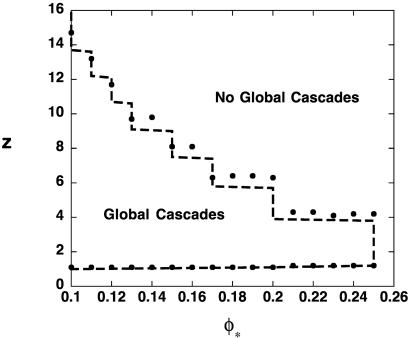
\includegraphics[height=0.8\textheight]{../figures/watts-fig-1}
            \caption{Watts 2002 Figure 1}
            \label{fig:watts-fig-1}
        \end{figure}
    \end{frame}
    
        \begin{frame}[BlankLogo]
            Larger Image: \url{https://github.com/chendaniely/gbcb_seminar_presentation_1/raw/master/figures/p_flipped_all.png}
        \end{frame}
    
    \begin{frame}[BlankLogo]
        \begin{figure}
            \centering
            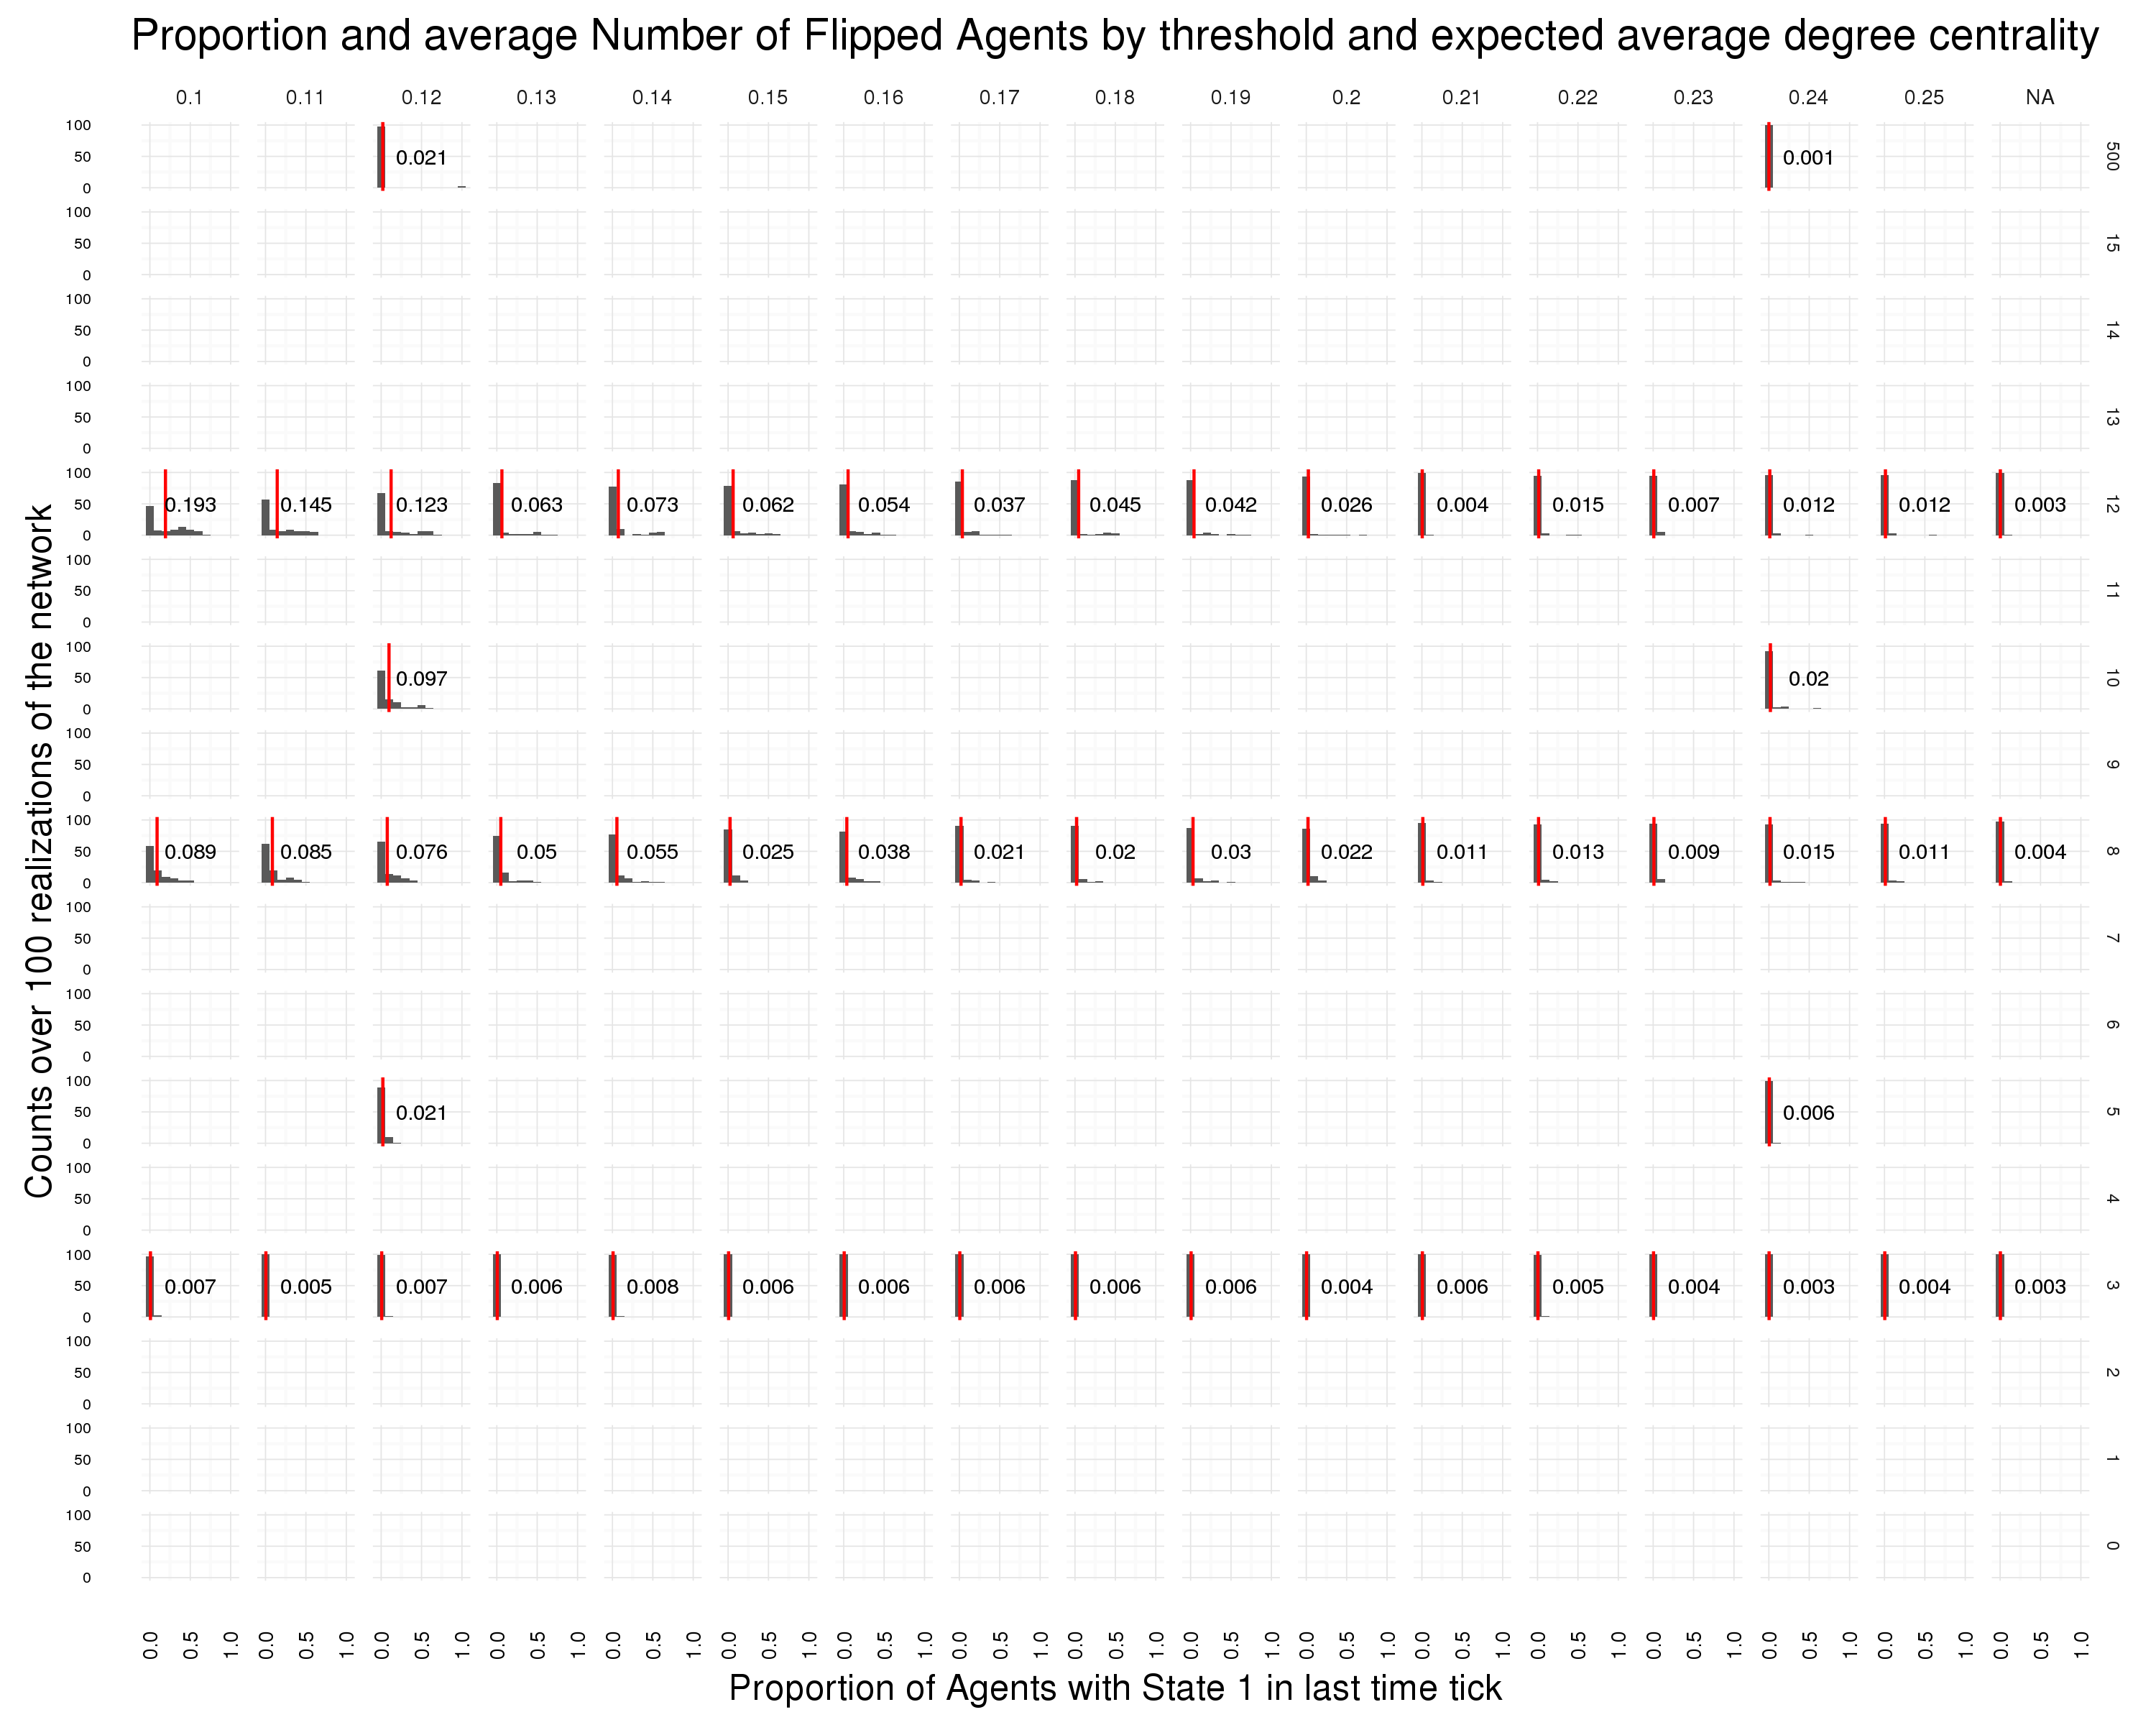
\includegraphics[width=0.75\linewidth]{../figures/p_flipped_all}
            \caption{}
            \label{fig:pflippedall}
        \end{figure}
    \end{frame}

\section{TRA}

\subsection{Expand the Watts Model}

    \begin{frame}[Basic2]\frametitle{Expand the Watts Model}
        The Watts model can be used to model any \textbf{binary outcome}.
        
        From a \textbf{public health} and \textbf{epidemiology} perspective,
        this outcome can be a particular \textbf{behavior or action}.
        \vspace{2mm}
        \begin{itemize}
            \item I ate a cookie.  Yes/No
        \end{itemize}
        
        \vspace{3mm}
        
        However, our decision making process is not that simple.
    \end{frame}

\subsection{Theory of Reasoned Action}

    \begin{frame}[Basic2]\frametitle{Theory of Reasoned Action (TRA)}
        Health behavior model

        \begin{itemize}
            \item Martin Fishbein and Icek Ajzen 1967
            \item Behavior is determined by an individual's intention
            \item Intention comes from an individual's attitudes and social context
            \item Attitudes and social context originates from a set of beliefs
        \end{itemize}
        
        \vspace{3mm}
        
        \textbf{beliefs} $\rightarrow$ (attitudes \& social context) $\rightarrow$ intention $\rightarrow$ behavior
        
    \end{frame}
    
    \begin{frame}[BlankLogo]
        % But first, let me take a selfie
    \end{frame}

    \begin{frame}[Basic2]\frametitle{TRA as Parallel Constraint Satisfaction}
        \begin{columns}
            \begin{column}{0.5\linewidth}

                        \vspace{7mm}

                        \begin{figure}
                            \centering
                            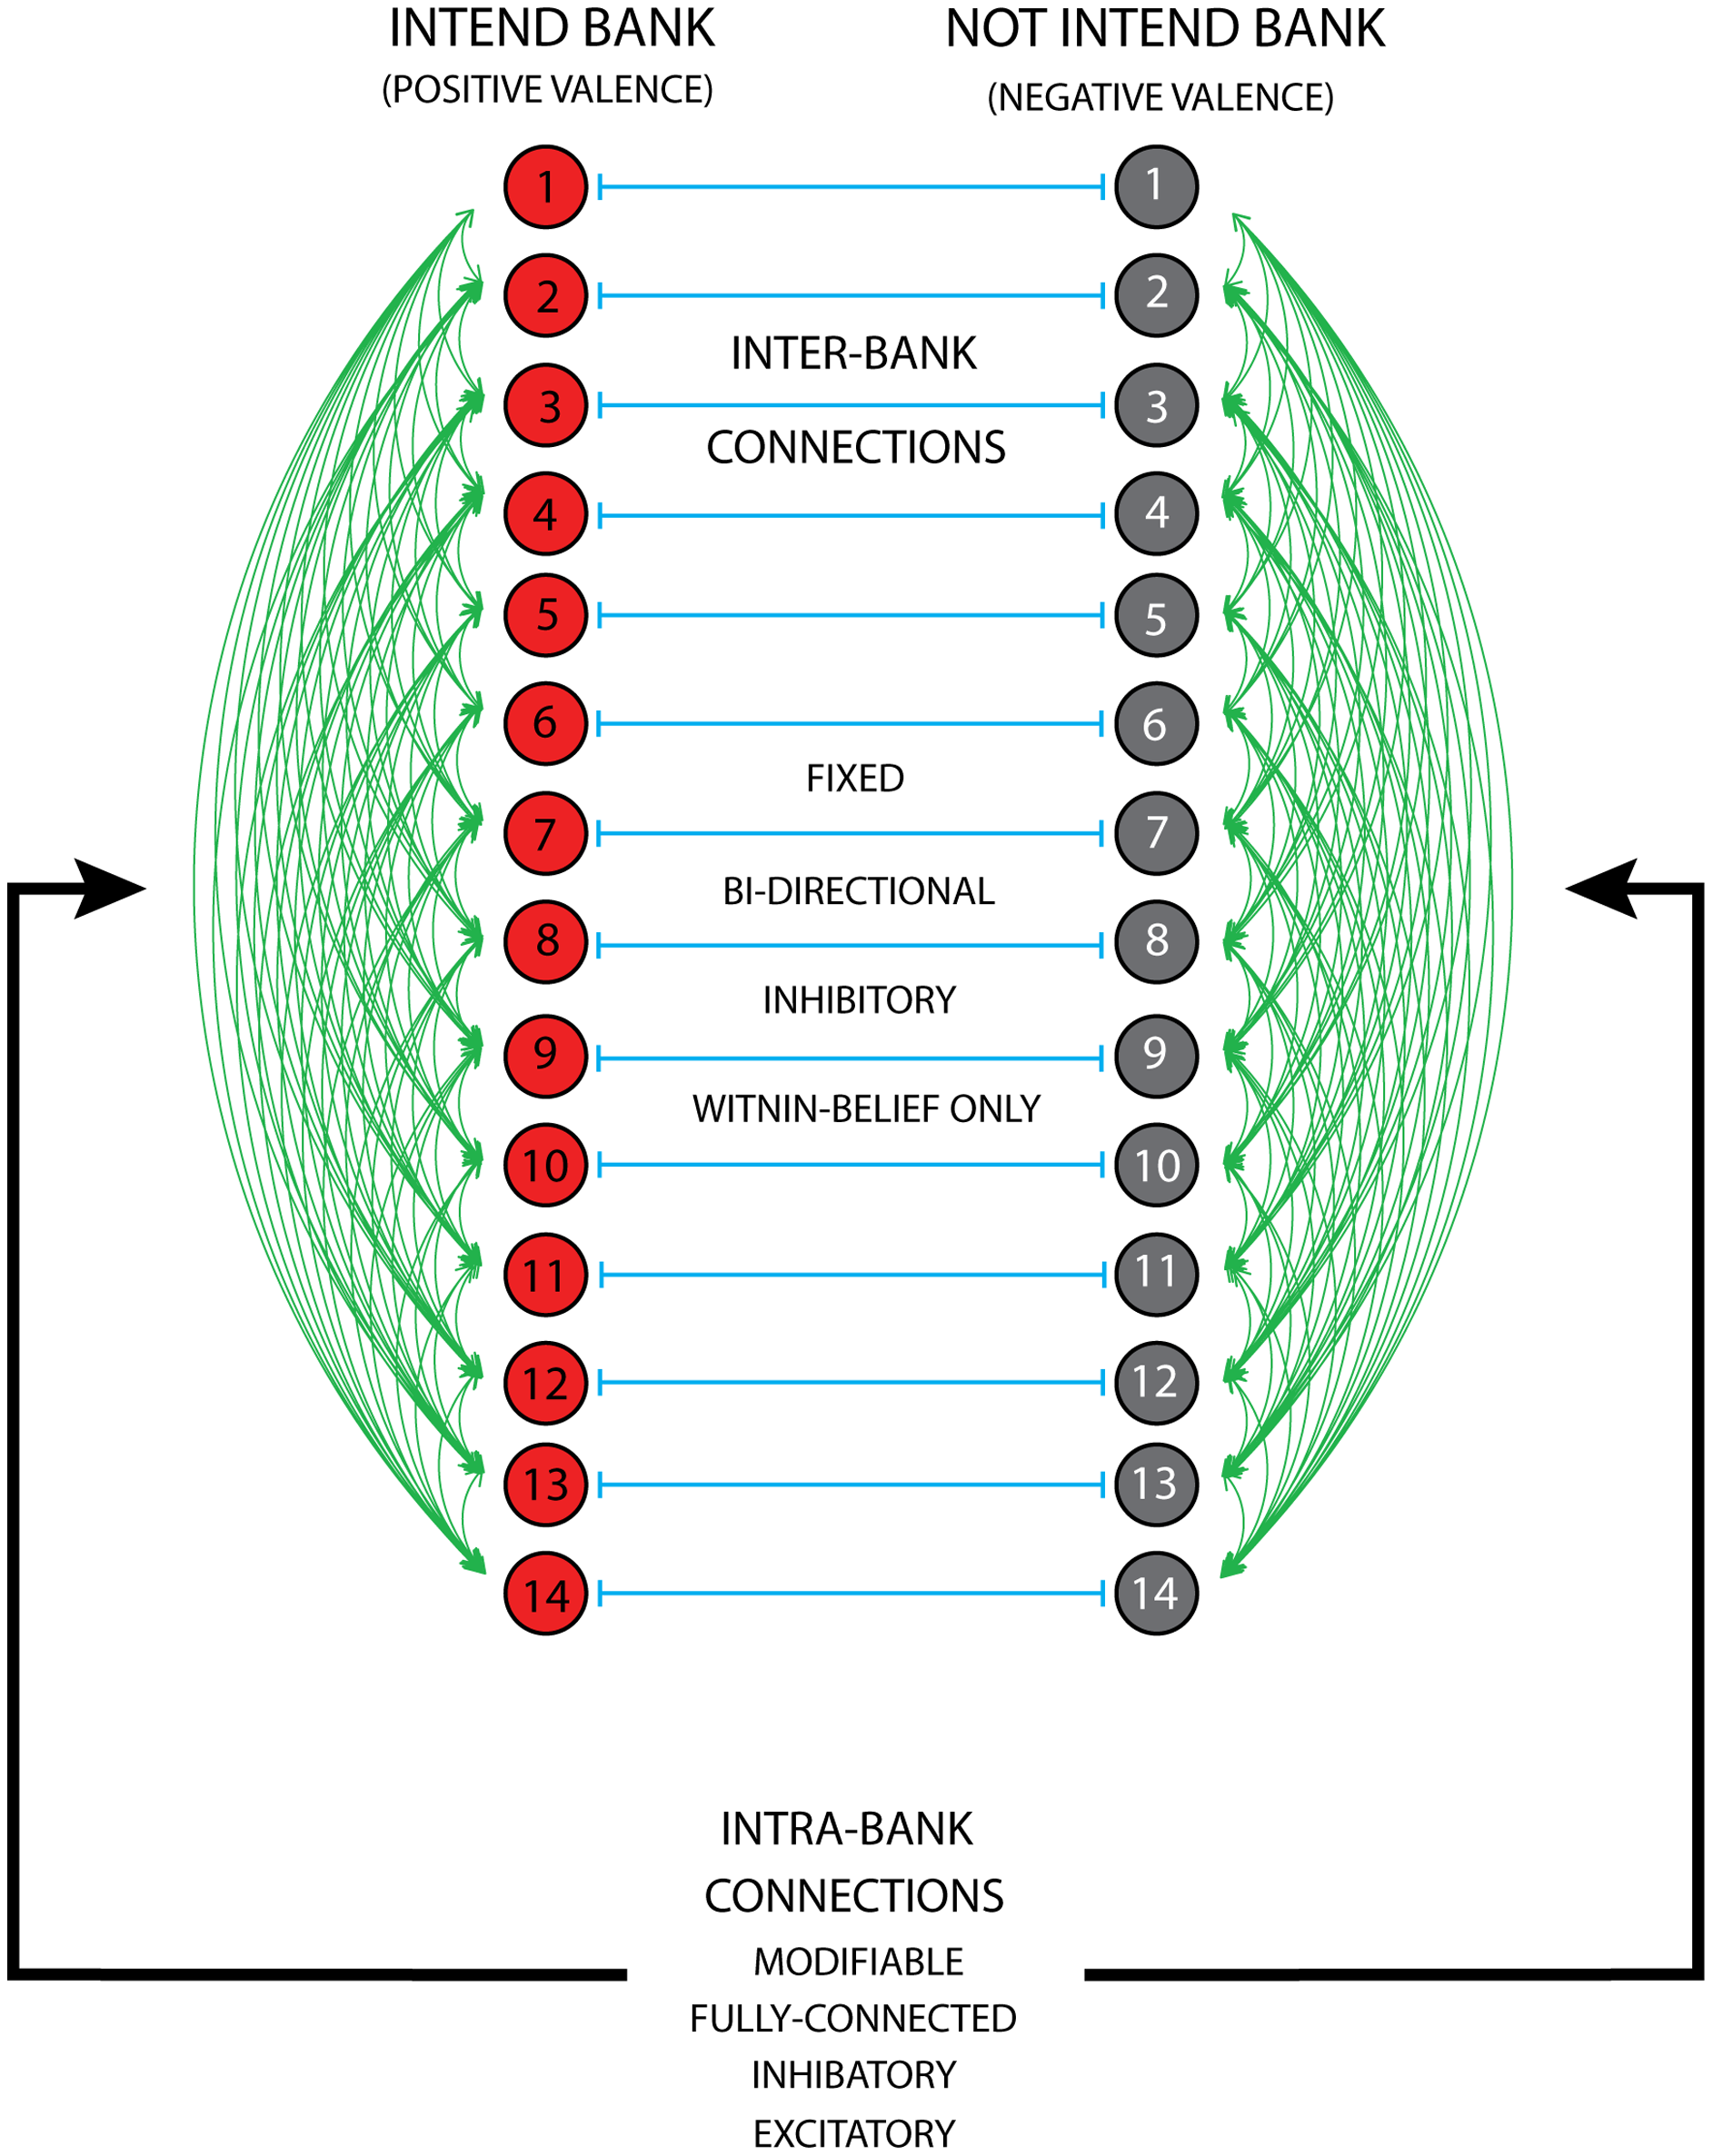
\includegraphics[height=0.7\textheight]{../figures/tra_nn}
                            \caption{Orr 2013 Figure 1}
                            \label{fig:trann}
                        \end{figure}
            \end{column}
            \begin{column}{0.5\linewidth}
                
                \vspace{7mm}
                
                \begin{figure}
                    \centering
                    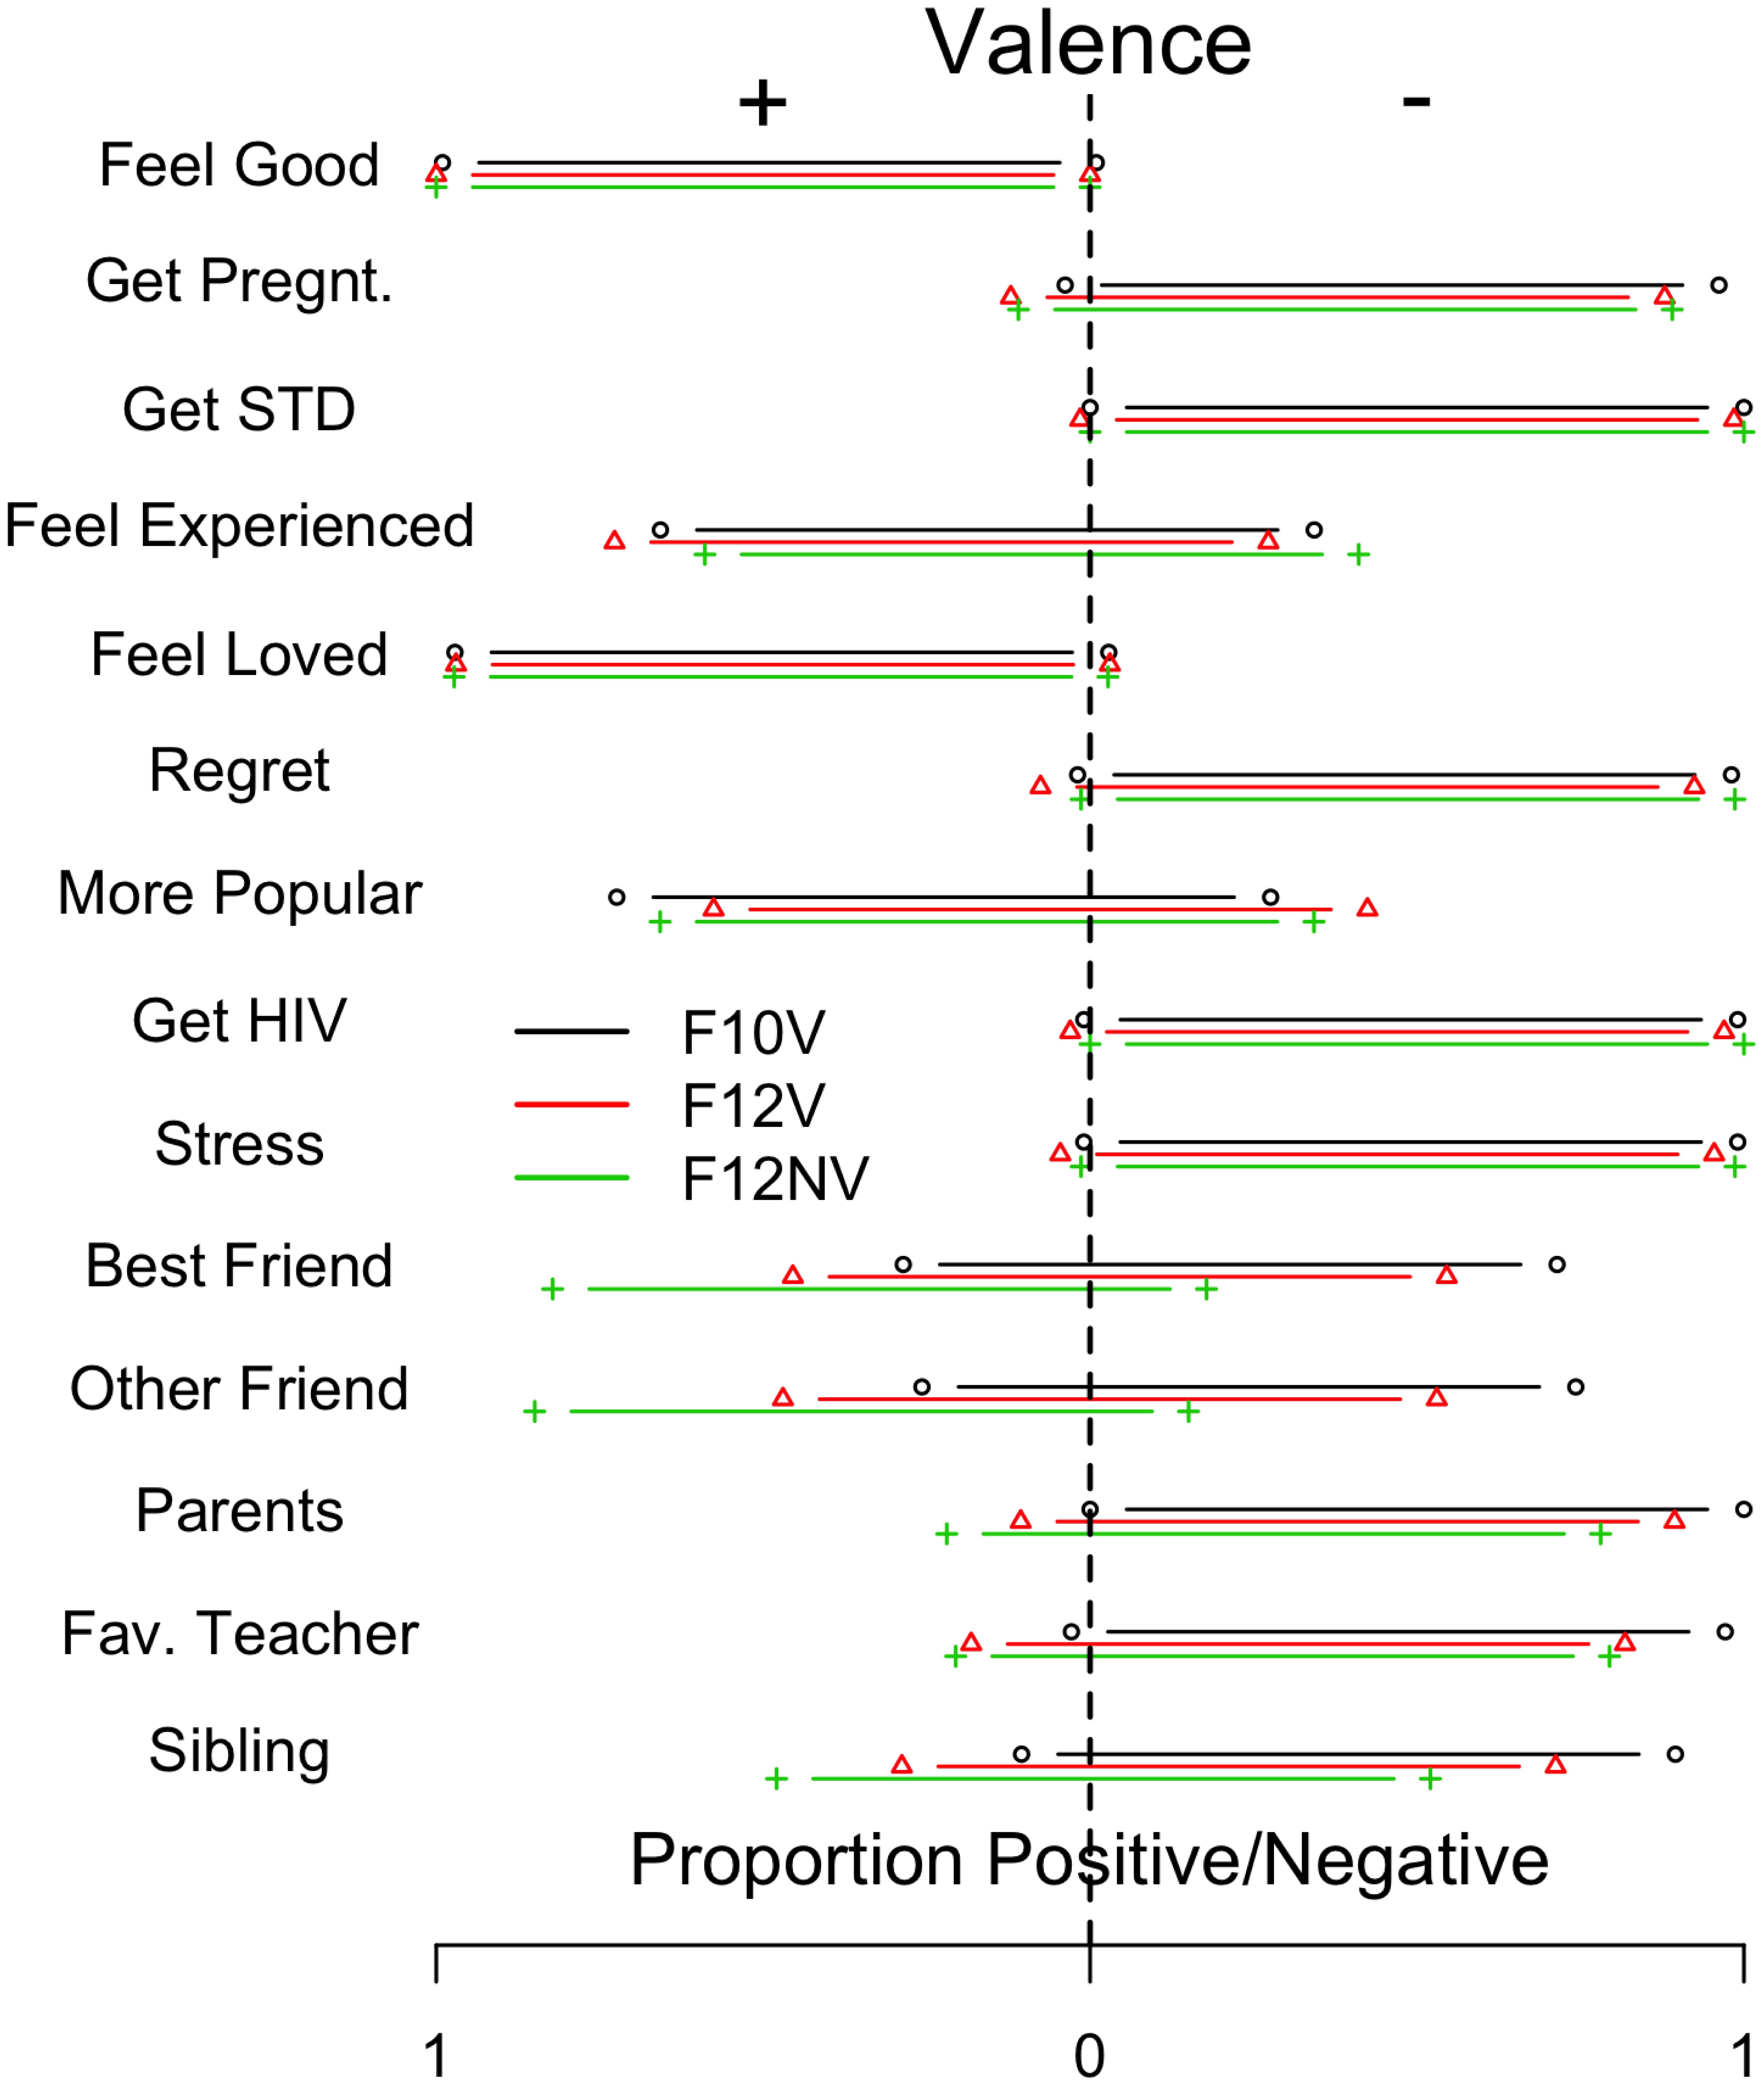
\includegraphics[height=0.7\textheight]{../figures/tra_example}
                    \caption{Orr 2013 Figure 2}
                \label{fig:traexample}
\end{figure}

            \end{column}
        \end{columns}
    \end{frame}

\section{Neural Networks}

\subsection{Neural Networks}

    \begin{frame}[Basic2]\frametitle{Neural Network}
        \begin{columns}
            \begin{column}{0.5\linewidth}
                \vspace{3mm}
                \footnotesize
                        \begin{itemize}
                            \item \textbf{Logistic regression}
                            \item The perceptron is a classic `simple' neural network.
                            \begin{itemize}
                                \item Feed-forward nerual network
                                \item \textbf{Recurrent}
                                \item ``deep learning''
                                \begin{itemize}
                                    \item AlphaGo vs Lee Sedol
                                    \item Self-driving cars
                                \end{itemize}
                            \end{itemize}
                            \item Psychological plausible decisions
                            \begin{itemize}
                                \item social processes
                                \item experience/ memory
                                \item influences/ dynamic
                            \end{itemize}
                        \end{itemize}
            \end{column}
            \begin{column}{0.5\linewidth}
                \vspace{7mm}
                \begin{figure}
                    \centering
                    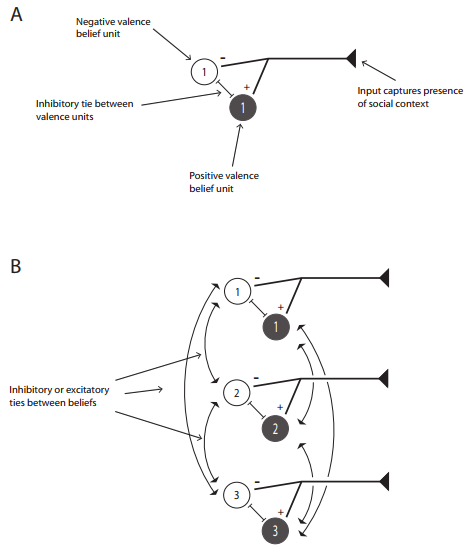
\includegraphics[width=0.7\linewidth]{../figures/orr_nn}
                    \caption{Orr 2014 Figure 1}
                    \label{fig:orrnn}
                    \end{figure}
            \end{column}
        \end{columns}
    \end{frame}

\subsection{Neural Network Visualization}

    \begin{frame}[Basic2]\frametitle{TensorFlow Visualization}
        
        \vspace{7mm}
        
        \begin{figure}
            \centering
            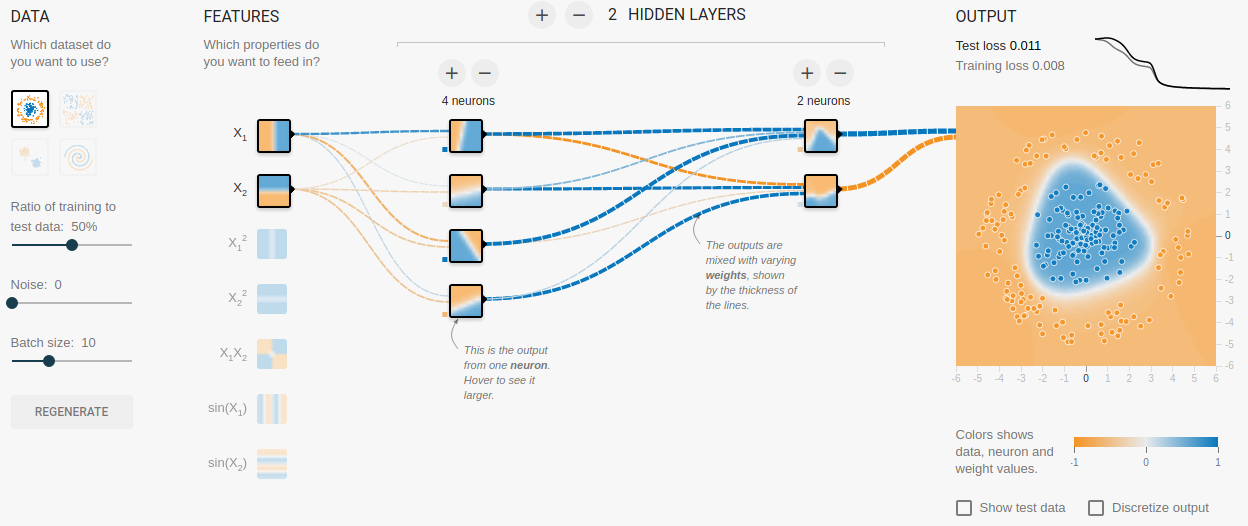
\includegraphics[width=0.9\linewidth]{../figures/tensorflow_visualization}
            \caption{}
            \label{fig:tensorflowvisualization}
        \end{figure}

        
        \url{http://playground.tensorflow.org/}
    \end{frame}

\section{Sims}

\subsection{Results}

    \begin{frame}[Blank]\frametitle{Results}
        \begin{columns}
            \begin{column}{0.5\linewidth}
                \vspace{-7mm}
                        \begin{figure}
                            \centering
                            \includegraphics[height=0.9\textheight]{../figures/mann_param_sweep}
                            \caption{}
                            \label{fig:mannparamsweep}
                        \end{figure}
            \end{column}
            \begin{column}{0.5\linewidth}
                Forthcoming Publication
                
                \begin{itemize}
                    \item parameter sweep on NN connections
                    \item no learning during simulation
                    \item 7750 Simulations
                    \item associativity
                    \begin{itemize}
                        \item  clustering of intention at the end of the simulation
                    \end{itemize}
                \end{itemize}
            \end{column}
        \end{columns}

    \end{frame}

\section{Fin}

\subsection{Future Directions and Questions}

    \begin{frame}[Basic2]\frametitle{Future Directions and Questions}
        \textbf{NSF}
        \begin{itemize}
            \item E-cigarettes
            \item Twitter
        \end{itemize}

        \textbf{NYT}: Shooting Scares Show a Nation Quick to Fear the Worst

       \textbf{Questions}:
     \begin{itemize}
            \item How to summarize the NN Simulation data
            \begin{itemize}
                \item Signal Decomposition/analysis
                \item t-SNE projections to look for community movement
            \end{itemize}
        \end{itemize}
    \end{frame}
    
\section{End}

\subsection{Forthcoming Works}
    \begin{frame}[Basic2] \frametitle{Forthcoming Works}
        \begin{enumerate}
            \item M. Orr, K. Zeimer, and D. Chen (Forthcoming, Fall 2016).
            \textit{Systems of Behavior and Human Health}. In S. Galea \& A. El-Sayed (Eds.),
            Systems Science and Population Health. Oxford University Press: Oxford, UK.

            \item M. Orr and D. Chen (Forthcoming, Fall 2016).
            \textit{Computational Models of Health Behavior}.
            In R. Vallacher, A. Nowak, and S. Read (Eds.),
            Computational Models in Social Psychology. Psychology Press/Routledge: New York.
        \end{enumerate}
    \end{frame}

\subsection{Thanks!}

    \begin{frame}[Basic2] \frametitle{Thanks!}
        \begin{itemize}
            \item Dennie Munson 
            \item Social and Decition Analytics Laboratory
        \end{itemize}

        \begin{itemize}
            \item Mark Orr, PhD (VT)
            \item Aaron Schroeder, PhD (VT)
            \item David Higdon, PHD (VT)
            \item Jacqueline Merrill PhD, MPH, RN, FAAN, FACMI (CU Nursing)
        \end{itemize}

        
\includegraphics[width=10mm]{../figures/nsf} \#1520359

    \end{frame}
    
        \begin{frame}[Basic2]\frametitle{GBCB!}
            \vspace{7mm}
            
            \begin{figure}
                \centering
                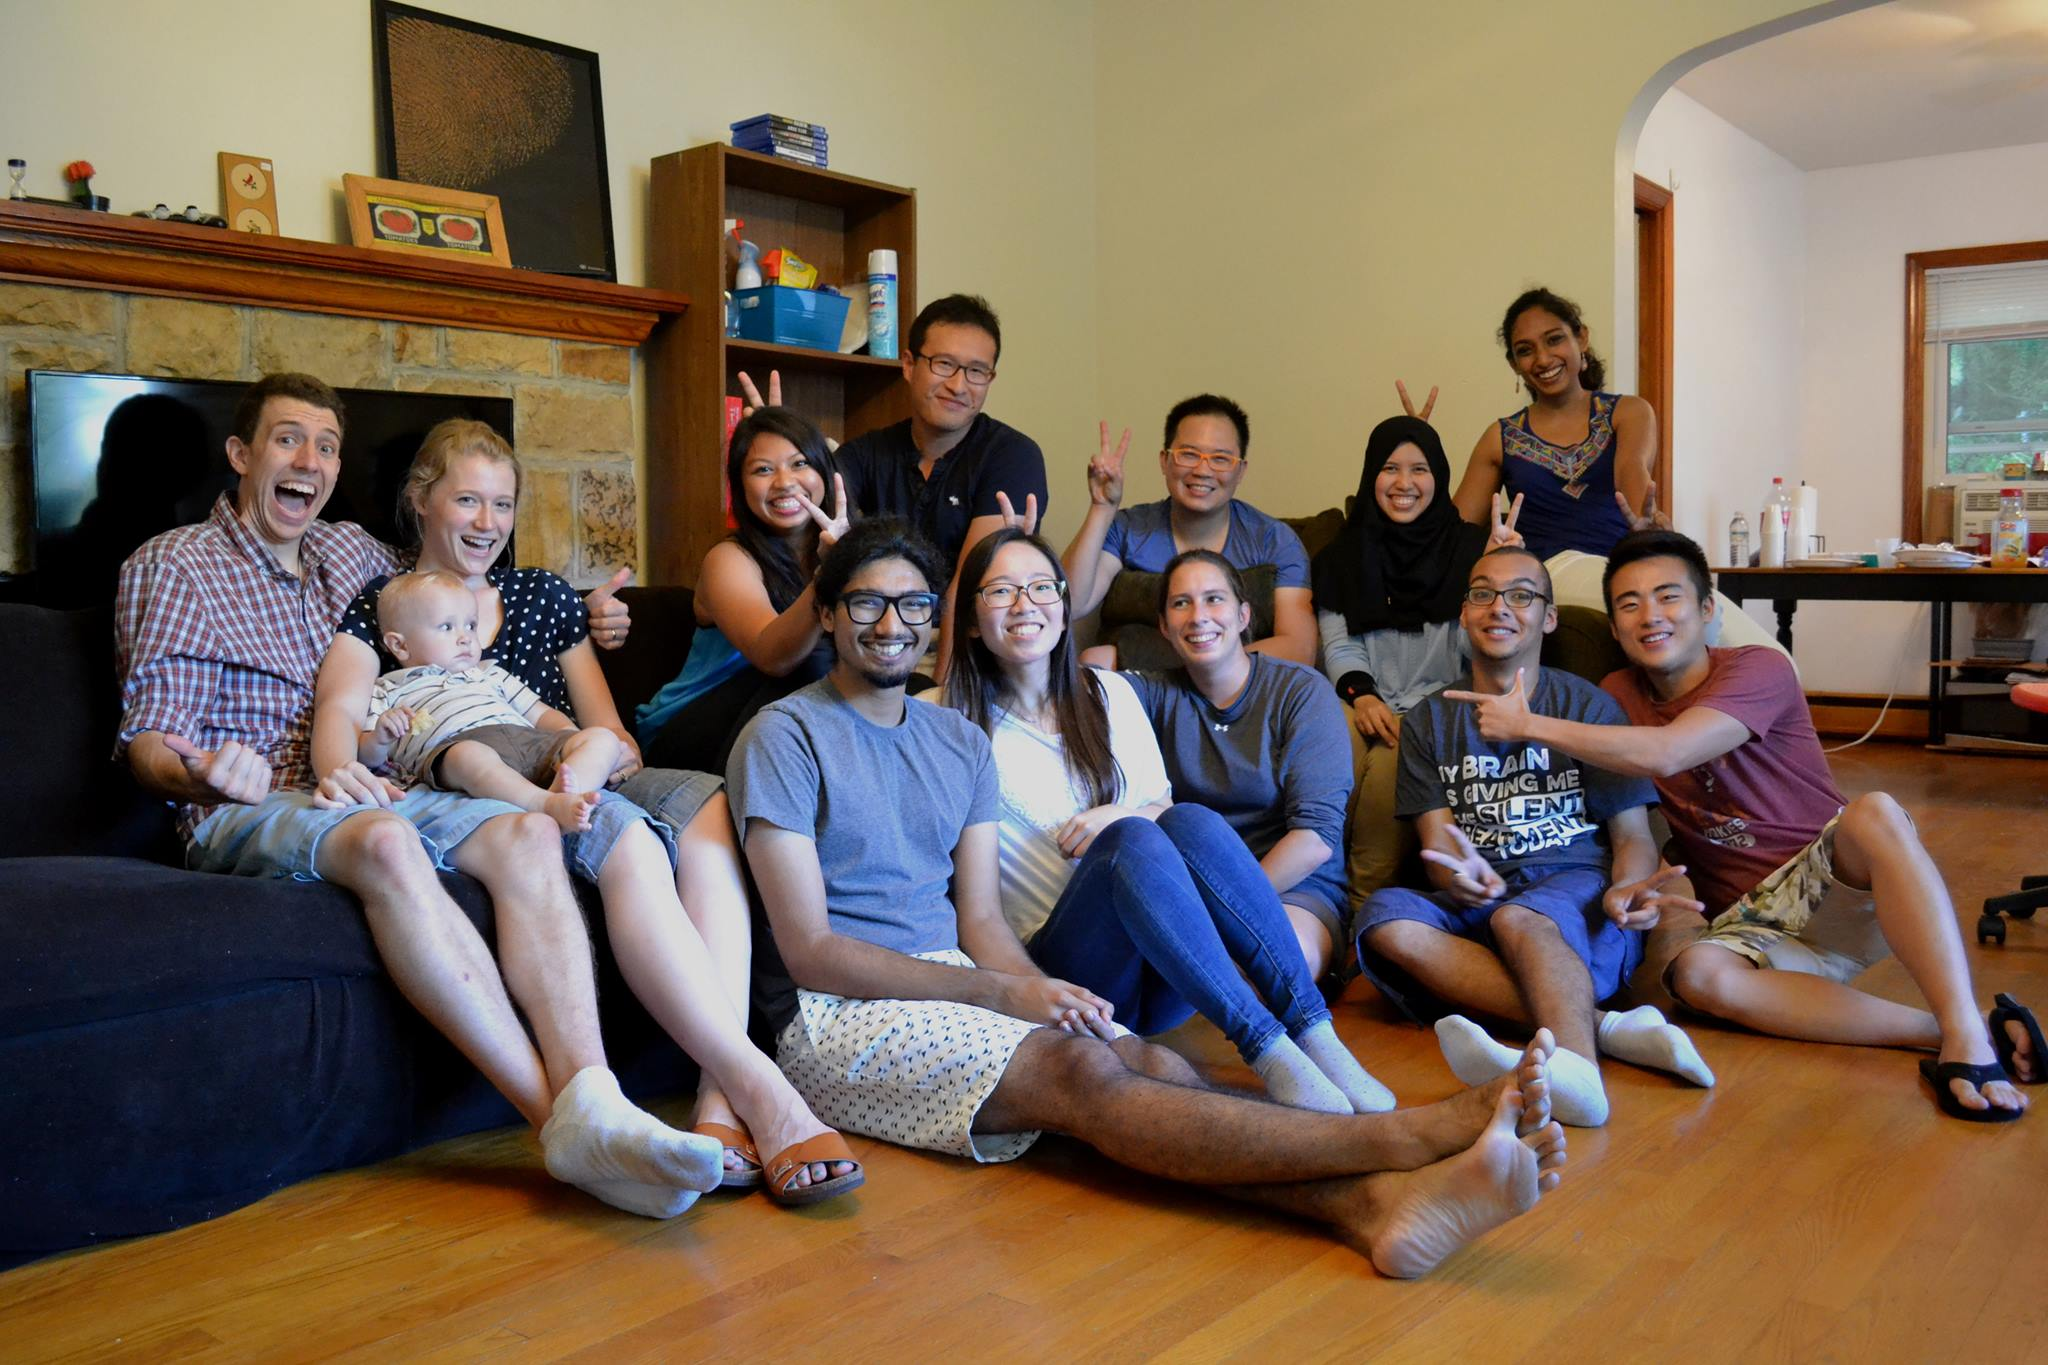
\includegraphics[width=0.7\linewidth]{../figures/gbcb}
                \caption{}
                \label{fig:gbcb}
            \end{figure}
            
        \end{frame}
    
    \begin{frame}[Basic2] \frametitle{Thanks!}
        \begin{columns}
            \begin{column}{0.5\textwidth}
                \vspace{7mm}
                
                \begin{figure}
                    \centering
                    
\includegraphics[height=0.7\textheight]{../figures/programming-comic-latex}
                    \caption{}
                    \label{fig:programming-comic-latex}
                \end{figure}
            \end{column}
            \begin{column}{0.5\textwidth}
                \vspace{7mm}
                
                \begin{figure}
                    \centering
                    
\includegraphics[width=0.9\linewidth]{../figures/latex_typesetting}
                    \caption{}
                    \label{fig:latextypesetting}
                \end{figure}
            \end{column}
        \end{columns}
    \end{frame}
    


\subsection{References}
    \begin{frame}[allowframebreaks, Blank]
            \frametitle{References}
            \nocite{*}
            \tiny
            \bibliographystyle{plain}
            \bibliography{bib}
    \end{frame}

\subsection{Links}
    \begin{frame}[Basic2] \frametitle{Thanks!}
       \begin{columns}
           \begin{column}{0.57\textwidth}
                \tiny
                
                \textbf{Slides}:\\
                    \url{https://github.com/chendaniely/gbcb_seminar_presentation_1}
                \vspace{2mm}
                \textbf{Code}:
                \begin{itemize}
                   %\item https://github.com/chendaniely/multi-agent-neural-network
                   %\item https://github.com/chendaniely/multidisciplinary-diffusion-model-experiments
                   \item \url{https://github.com/chendaniely/mann2}
                   \item \url{https://github.com/chendaniely/mann2\_simulations}
                   \item \url{https://github.com/chendaniely/mann2\_analysis}
                \end{itemize}
                
                
\includegraphics[width=7mm]{../figures/font-awesome_4-6-3_twitter_256_0_007dff_none}
                @chendaniely
                
                \includegraphics[width=7mm]{../figures/brandico_2014-04-07_github_256_0_2c3e50_none}
                www.github.com/chendaniely
            \end{column}
            \begin{column}{0.43\textwidth}
                \vspace{10mm}

                \begin{figure}
                    \centering
                    \includegraphics[width=0.8\linewidth]{../figures/pandas_for_everyone}
                    \caption{}
                    \label{fig:pandasforeveryone}
                \end{figure}
            \end{column}
        \end{columns}
    \end{frame}

\end{document}

http://www.nytimes.com/2016/08/30/us/shooting-scares-show-a-nation-quick-to-fear-the-worst.html?action=click&contentCollection=us&region=rank&module=package&version=highlights&contentPlacement=1&pgtype=sectionfront

% abstract
Binary decision models with externalities is a class of models that describe individuals making a simple binary choose,
whose decision depends on other people.
This class of models is generalizable to infectious diseases, decision making, information spread, fads, riots, etc.
However, binary decision models are not rich enough to describe the complex process of human attitude formation that eventually lead to behaviors.
The Theory of Reasoned Action states that behaviors stem from a series of beliefs.
This theory is used as the computational framework for constraint satisfaction artificial neural networks, which allows us to model psychologically plausible decisions on an individual level.
This model can be combined with agent-based models, which model health behavior at a population level in order to add psychology into a dynamic social network framework.
This new framework for epidemiological modeling of health behaviors where the agents may exhibit psychological plausible decisions all us to study the spreading of ideas within a social network.
This will give us insights as to what drives behavioral risk factors for population health behaviors.

